        %%******************************************%%
        %%                                          %%
        %%        Modello di tesi di laurea         %%
        %%            di Andrea Giraldin            %%
        %%                                          %%
        %%             2 novembre 2012              %%
        %%                                          %%
        %%******************************************%%


% I seguenti commenti speciali impostano:
% 1. 
% 2. PDFLaTeX come motore di composizione;
% 3. tesi.tex come documento principale;
% 4. il controllo ortografico italiano per l'editor.

% !TEX encoding = UTF-8
% !TEX TS-program = pdflatex
% !TEX root = tesi.tex
% !TEX spellcheck = it-IT

\documentclass[10pt,                    % corpo del font principale
               a4paper,                 % carta A4
               twoside,                 % impagina per fronte-retro
               openright,               % inizio capitoli a destra
               english,                 
               italian,                 
               ]{book}    

%**************************************************************
% Importazione package
%************************************************************** 

%\usepackage{amsmath,amssymb,amsthm}    % matematica

\usepackage[T1]{fontenc}                % codifica dei font:
                                        % NOTA BENE! richiede una distribuzione *completa* di LaTeX
\usepackage{lmodern}

\usepackage[utf8]{inputenc}             % codifica di input; anche [latin1] va bene
                                        % NOTA BENE! va accordata con le preferenze dell'editor

\usepackage[english, italian]{babel}    % per scrivere in italiano e in inglese;
                                        % l'ultima lingua (l'italiano) risulta predefinita

\usepackage{bookmark}                   % segnalibri

\usepackage{caption}                    % didascalie

\usepackage{chngpage,calc}              % centra il frontespizio

\usepackage{csquotes}                   % gestisce automaticamente i caratteri (")

\usepackage{emptypage}                  % pagine vuote senza testatina e piede di pagina

\usepackage{epigraph}			% per epigrafi

\usepackage{eurosym}                    % simbolo dell'euro

%\usepackage{indentfirst}               % rientra il primo paragrafo di ogni sezione

\usepackage{graphicx}                   % immagini

\usepackage{hyperref}                   % collegamenti ipertestuali

\usepackage[binding=5mm]{layaureo}      % margini ottimizzati per l'A4; rilegatura di 5 mm

\usepackage{listings}                   % codici

\usepackage{microtype}                  % microtipografia

\usepackage{mparhack,fixltx2e,relsize}  % finezze tipografiche

\usepackage{nameref}                    % visualizza nome dei riferimenti                                      

\usepackage[font=small]{quoting}        % citazioni

\usepackage{subfig}                     % sottofigure, sottotabelle

\usepackage[italian]{varioref}          % riferimenti completi della pagina

\usepackage[dvipsnames,table]{xcolor}         % colori

\usepackage{booktabs}                   % tabelle                                       
\usepackage{tabularx}                   % tabelle di larghezza prefissata                                    
\usepackage{longtable}                  % tabelle su più pagine                                        
\usepackage{ltxtable}                   % tabelle su più pagine e adattabili in larghezza

\usepackage[toc, acronym]{glossaries}   % glossario
                                        % per includerlo nel documento bisogna:
                                        % 1. compilare una prima volta tesi.tex;
                                        % 2. eseguire: makeindex -s tesi.ist -t tesi.glg -o tesi.gls tesi.glo
                                        % 3. eseguire: makeindex -s tesi.ist -t tesi.alg -o tesi.acr tesi.acn
                                        % 4. compilare due volte tesi.tex.

\usepackage[backend=biber,style=verbose-ibid,hyperref,backref]{biblatex}
                                        % eccellente pacchetto per la bibliografia; 
                                        % produce uno stile di citazione autore-anno; 
                                        % lo stile "numeric-comp" produce riferimenti numerici
                                        % per includerlo nel documento bisogna:
                                        % 1. compilare una prima volta tesi.tex;
                                        % 2. eseguire: biber tesi
                                        % 3. compilare ancora tesi.tex.
\usepackage{placeins}
\usepackage{listings}
% Copyright 2017 Sergei Tikhomirov, MIT License
% https://github.com/s-tikhomirov/solidity-latex-highlighting/

\usepackage{listings, xcolor}

\definecolor{verylightgray}{rgb}{.97,.97,.97}

\lstdefinelanguage{Solidity}{
	keywords=[1]{anonymous, assembly, assert, balance, break, call, callcode, case, catch, class, constant, continue, constructor, contract, debugger, default, delegatecall, delete, do, else, emit, event, experimental, export, external, false, finally, for, function, gas, if, implements, import, in, indexed, instanceof, interface, internal, is, length, library, log0, log1, log2, log3, log4, memory, modifier, new, payable, pragma, private, protected, public, pure, push, require, return, returns, revert, selfdestruct, send, solidity, storage, struct, suicide, super, switch, then, this, throw, transfer, true, try, typeof, using, value, view, while, with, addmod, ecrecover, keccak256, mulmod, ripemd160, sha256, sha3}, % generic keywords including crypto operations
	keywordstyle=[1]\color{blue}\bfseries,
	keywords=[2]{address, bool, byte, bytes, bytes1, bytes2, bytes3, bytes4, bytes5, bytes6, bytes7, bytes8, bytes9, bytes10, bytes11, bytes12, bytes13, bytes14, bytes15, bytes16, bytes17, bytes18, bytes19, bytes20, bytes21, bytes22, bytes23, bytes24, bytes25, bytes26, bytes27, bytes28, bytes29, bytes30, bytes31, bytes32, enum, int, int8, int16, int24, int32, int40, int48, int56, int64, int72, int80, int88, int96, int104, int112, int120, int128, int136, int144, int152, int160, int168, int176, int184, int192, int200, int208, int216, int224, int232, int240, int248, int256, mapping, string, uint, uint8, uint16, uint24, uint32, uint40, uint48, uint56, uint64, uint72, uint80, uint88, uint96, uint104, uint112, uint120, uint128, uint136, uint144, uint152, uint160, uint168, uint176, uint184, uint192, uint200, uint208, uint216, uint224, uint232, uint240, uint248, uint256, var, void, ether, finney, szabo, wei, days, hours, minutes, seconds, weeks, years},	% types; money and time units
	keywordstyle=[2]\color{teal}\bfseries,
	keywords=[3]{block, blockhash, coinbase, difficulty, gaslimit, number, timestamp, msg, data, gas, sender, sig, value, now, tx, gasprice, origin},	% environment variables
	keywordstyle=[3]\color{violet}\bfseries,
	identifierstyle=\color{black},
	sensitive=false,
	comment=[l]{//},
	morecomment=[s]{/*}{*/},
	commentstyle=\color{gray}\ttfamily,
	stringstyle=\color{red}\ttfamily,
	morestring=[b]',
	morestring=[b]"
}

\lstset{
	language=Solidity,
	backgroundcolor=\color{verylightgray},
	extendedchars=true,
	basicstyle=\footnotesize\ttfamily,
	showstringspaces=false,
	showspaces=false,
	numbers=left,
	numberstyle=\footnotesize,
	numbersep=9pt,
	tabsize=2,
	breaklines=true,
	showtabs=false,
	captionpos=b
}
\lstdefinelanguage{Kotlin}{
  comment=[l]{//},
  commentstyle={\color{gray}\ttfamily},
  emph={delegate, filter, first, firstOrNull, forEach, lazy, map, mapNotNull, println, return@},
  emphstyle={\color{OrangeRed}},
  identifierstyle=\color{black},
  keywords={abstract, actual, as, as?, break, by, class, companion, continue, data, do, dynamic, else, enum, expect, false, final, for, fun, get, if, import, in, interface, internal, is, null, object, override, package, private, public, return, set, super, suspend, this, throw, true, try, typealias, val, var, vararg, when, where, while},
  keywordstyle={\color{NavyBlue}\bfseries},
  morecomment=[s]{/*}{*/},
  morestring=[b]",
  morestring=[s]{"""*}{*"""},
  ndkeywords={@Deprecated, @JvmField, @JvmName, @JvmOverloads, @JvmStatic, @JvmSynthetic, Array, Byte, Double, Float, Int, Integer, Iterable, Long, Runnable, Short, String},
  ndkeywordstyle={\color{BurntOrange}\bfseries},
  sensitive=true,
  stringstyle={\color{ForestGreen}\ttfamily},
}
%**************************************************************
% file contenente le impostazioni della tesi
%**************************************************************

%**************************************************************
% Frontespizio
%**************************************************************

% Autore
\newcommand{\myName}{Matteo Infantino}                                    
\newcommand{\myTitle}{Studio e implementazione di smart contract per la piattaforma Ethereum in ambito contact tracing}

% Tipo di tesi                   
\newcommand{\myDegree}{Tesi di laurea triennale}

% Università             
\newcommand{\myUni}{Università degli Studi di Padova}

% Facoltà       
\newcommand{\myFaculty}{Corso di Laurea in Informatica}

% Dipartimento
\newcommand{\myDepartment}{Dipartimento di Matematica "Tullio Levi-Civita"}

% Titolo del relatore
\newcommand{\profTitle}{Prof. }

% Relatore
\newcommand{\myProf}{Lamberto Ballan}

% Luogo
\newcommand{\myLocation}{Padova}

% Anno accademico
\newcommand{\myAA}{2019-2020}

% Data discussione
\newcommand{\myTime}{Luglio 2020}


%**************************************************************
% Impostazioni di impaginazione
% see: http://wwwcdf.pd.infn.it/AppuntiLinux/a2547.htm
%**************************************************************

\setlength{\parindent}{14pt}   % larghezza rientro della prima riga
\setlength{\parskip}{0pt}   % distanza tra i paragrafi


%**************************************************************
% Impostazioni di biblatex
%**************************************************************
\bibliography{bibliografia} % database di biblatex 

\defbibheading{bibliography} {
    \cleardoublepage
    \phantomsection 
    \addcontentsline{toc}{chapter}{\bibname}
    \chapter*{\bibname\markboth{\bibname}{\bibname}}
}

\setlength\bibitemsep{1.5\itemsep} % spazio tra entry

\DeclareBibliographyCategory{opere}
\DeclareBibliographyCategory{web}

\addtocategory{opere}{womak:lean-thinking}
\addtocategory{web}{site:agile-manifesto}

\defbibheading{opere}{\section*{Riferimenti bibliografici}}
\defbibheading{web}{\section*{Siti Web consultati}}


%**************************************************************
% Impostazioni di caption
%**************************************************************
\captionsetup{
    tableposition=top,
    figureposition=bottom,
    font=small,
    format=hang,
    labelfont=bf
}

%**************************************************************
% Impostazioni di glossaries
%**************************************************************

%**************************************************************
% Acronimi
%**************************************************************
\renewcommand{\acronymname}{Acronimi e abbreviazioni}

\newacronym[description={\glslink{apig}{Application Program Interface}}]
    {api}{API}{Application Program Interface}

\newacronym[description={\glslink{umlg}{Unified Modeling Language}}]
    {uml}{UML}{Unified Modeling Language}

%**************************************************************
% Glossario
%**************************************************************
%\renewcommand{\glossaryname}{Glossario}

\newglossaryentry{turn over}
{
    name=\glslink{turn over}{Turn over aziendale},
    text=Turn over,
    sort=turn over,
    description={Tasso di ricambio del personale, ovvero il flusso di persone in ingresso e in uscita da un'azienda}
}

\newglossaryentry{big data}
{
    name=\glslink{big data}{Big data},
    text=big data,
    sort=Big Data,
    description={Tecniche e metodologie di analisi di grandi quantità di dati ovvero la capacità di estrapolare, analizzare e mettere in relazione un’enorme mole di dati eterogenei, strutturati e non strutturati, per scoprire i legami tra fenomeni diversi e prevedere quelli futuri. Si parla di big data quando si ha un insieme talmente grande e complesso di dati che richiede la definizione di nuovi strumenti e metodologie per estrapolare, gestire e processare informazioni entro un tempo ragionevole}
}

\newglossaryentry{cloud computing}
{
    name=\glslink{cloud computing}{Cloud computing},
    text=cloud computing,
    sort=Cloud Computing,
    description={Con il termine Cloud Computing (ing. “nuvola informatica”) si indica un
paradigma di erogazione di servizi offerti on demand da un fornitore ad un cliente finale
attraverso la rete Internet}
}

\newglossaryentry{internet of things}
{
    name=\glslink{internet of things}{Internet of things},
    text=internet of things,
    sort=Internet of Things,
    description={Nelle telecomunicazioni, Internet of things (internet degli oggetti) è
il modo di riferirsi all’estensione di Internet al mondo degli oggetti e dei luoghi concreti.
Al giorno d’oggi infatti sempre più oggetti comuni hanno la possibilità di interfacciarsi
con il web, a partire da lavatrici, frigoriferi per arrivare a tutta la casa controllabile e
accessibile da remoto}
}

\newglossaryentry{information and communication technology}
{
    name=\glslink{information and communication technology}{Information and Communication Technology},
    text=information and communication technology,
    sort=Information and Communication Technology,
    description={Con ICT si indica il settore legato allo sviluppo delle strutture internet e
mobile, in particolare per ciò che riguarda gli aspetti di progettazione e realizzazione delle
componenti fisiche o di quelle digitali. Più in generale, le ICT comprendono l’insieme
dei metodi e delle tecniche utilizzate nella trasmissione, ricezione ed elaborazione di dati
e informazioni digitali, ampiamente diffusesi a partire dalla cosiddetta Terza rivoluzione
industriale: hardware,software e tecnologie ICT costituiscono oggi le tre componenti
principali delsettore IT}
}

\newglossaryentry{contact tracing}
{
    name=\glslink{contact tracing}{Contact tracing},
    text=contact tracing,
    sort=contact tracing,
    description={Il contact tracing è il tracciamento dei contatti nell'ambito della sanità pubblica, tramite il quale si identificano le persone che potrebbero essere venute a contatto con una persona infetta. Nell'ambito informatico con applicazione per il contact tracing si intende un programma tipicamente per smartphone che raccolga le informazioni relative ai contatti tra utenti}
}

\newglossaryentry{bluetooth LE}
{
    name=\glslink{bluetooth LE}{Bluetooth LE},
    text=bluetooth LE,
    sort=bluetooth LE,
    description={Il bluetooth LE è una tecnologia wireless con consumi energetici notevolmente ridotti rispetto al bluetooth classico, seppur con intervalli di comunicazione simili. Le sue caratteristiche si adattano a molteplici applicazioni che richiedono elevati utilizzi nel tempo del bluetooth, come per il contact tracing}
}

\newglossaryentry{UML}
{
    name=\glslink{UML}{UML},
    text=UML,
    sort=uml,
    description={in ingegneria del software \emph{UML, Unified Modeling Language} (ing. linguaggio di modellazione unificato) è un linguaggio di modellazione e specifica basato sul paradigma object-oriented. L'\emph{UML} svolge un'importantissima funzione di ``lingua franca'' nella comunità della progettazione e programmazione a oggetti. Gran parte della letteratura di settore usa tale linguaggio per descrivere soluzioni analitiche e progettuali in modo sintetico e comprensibile a un vasto pubblico}
}

\newglossaryentry{distributed ledger}
{
    name=\glslink{distributed ledger}{Distributed ledger},
    text=distributed ledger,
    sort=Distributed ledger,
    description={Il distributed ledger è un database condiviso e sincronizzato attraverso svariati nodi. Ogni nodo è autorizzato ad aggiornare il ledger in modo indipendente ma sotto il controllo consensuale degli altri. Non vi è un'autorità centrale come nei database tradizionali, ma l'incorrutibilità è garantita da un algoritmo di consenso}
}

\newglossaryentry{algoritmo di consenso}
{
    name=\glslink{algoritmo di consenso}{Algoritmo di consenso},
    text=algoritmo di consenso,
    sort=algoritmo di consenso,
    description={Un algoritmo di consenso è un meccanismo attraverso il quale i nodi assicurano la validazione di un blocco nella rete. È fondamentale nelle blockchain perché la mancanza di un ente che convalidi le transazioni deve coincidere con la sicurezza che le transazioni avvengano correttamente e le regole del protocollo siano seguite. Gli algorimi di consenso più conosciuti sono il Proof of Work e il Proof of Stake}
}

\newglossaryentry{single point of failure}
{
    name=\glslink{single point of failure}{Single point of failure},
    text=single point of failure,
    sort=single point of failure,
    description={Un single point of failure è un singolo punto del sistema il cui malfunzionanto può causare problemi all'intera operatività}
}

\newglossaryentry{permissionless}
{
    name=\glslink{permissionless}{Permissionless},
    text=permissionless,
    sort=Permissionless,
    description={Una blockchain che viene così definita non richiede
alcuna autorizzazione per poter accedere alla rete, eseguire delle transazioni o partecipare
alla verifica e creazione di un nuovo blocco}
}

\newglossaryentry{permissioned}
{
    name=\glslink{permissioned}{Permissioned},
    text=permissioned,
    sort=permissioned,
    description={Una blockchain che viene così definita permette solo a utenti autenticati e autorizzati di accedere alla rete, eseguire delle transazioni o partecipare alla verifica e creazione di un nuovo blocco}
}

\newglossaryentry{miner}
{
    name=\glslink{miner}{Miner},
    text=miner,
    sort=miner,
    description={In una blockchain con algoritmo di consenso Proof of Work, si definisce miner un nodo che risolve i problemi computazionali richiesti per la validazione di un blocco, dietro un compenso ricevuto a lavoro ultimato}
}

\newglossaryentry{Bitcoin}
{
    name=\glslink{Bitcoin}{Bitcoin},
    text=Bitcoin,
    sort=Bitcoin,
    description={Bitocoin è una blockchain creata nel 2009 da Satoshi Nakamoto che utilizza l'omonima criptovaluta. Utilizza un ledger distribuito fra i nodi per tenere traccia delle transazioni, validate tramite algoritmo Proof of Work}
}

\newglossaryentry{Ethereum}
{
    name=\glslink{Ethereum}{Ethereum},
    text=Ethereum,
    sort=Ethereum,
    description={Piattaforma decentralizzata ideata da Vitalik Buterik nel 2015, famosa per la possibilità di eseguire smart contracts in blockchain}
}

\newglossaryentry{proof of work}
{
    name=\glslink{proof of work}{Proof of work},
    text=proof of work,
    sort=proof of work,
    description={Algoritmo di consenso utilizzato da diverse criptovalute, come Bitcoin,
Ethereum e Litecoin per raggiungere un accordo decentralizzato tra diversi nodi nel
processo di aggiunta di un blocco specifico alla blockchain. Tale algoritmo obbliga i miners
a risolvere dei problemi matematici estremamente complessi e computazionalmente
difficili per poter aggiungere blocchi alla blockchain}
}

\newglossaryentry{double spending}
{
    name=\glslink{double spending}{Double spending},
    text=double spending,
    sort=double spending,
    description={Il double spending è una potenziale criticità delle criptovalute per cui lo stesso token digitale viene speso più di una volta}
}

\newglossaryentry{proof of stake}
{
    name=\glslink{proof of stake}{Proof of stake},
    text=proof of stake,
    sort=proof of stake,
    description={Algoritmo di consenso basato sul possesso di criptovalute: gli account con un gran numero di token hanno più possibilità di generare un blocco valido. È meno utilizzato rispetto al Proof of Work, ma è in grande sviluppo per via di numerosi vantaggi rispetto agli altri algoritmi di consenso, come la scalabilità e il minor costo e consumo energetico}
}

\newglossaryentry{token}
{
    name=\glslink{token}{Token},
    text=token,
    sort=token,
    description={In blockchain un token è un gettone virtuale emesso da un'organizzazione che rappresenta un'unità di valore}
}

\newglossaryentry{turing completi}
{
    name=\glslink{turing completi}{Linguaggio Turing completo},
    text=Turing completi,
    sort=turing-completi,
    description={Un linguaggio è detto Turing completo quando è in grado di eseguire qualunque programma che una macchina di Turing può esegiore, dato sufficiente tempo e memoria}
}

\newglossaryentry{applicazioni decentralizzate}
{
    name=\glslink{applicazioni decentralizzate}{Applicazioni decentralizzate},
    text=applicazioni decentralizzate,
    sort=applicazioni decentralizzate,
    description={Un'applicazione decentralizzata è un programma eseguito su un sistema distribuito come le blockchain}
}

\newglossaryentry{criptovaluta}
{
    name=\glslink{criptovaluta}{Criptovaluta},
    text=criptovaluta,
    sort=criptovaluta,
    description={La criptovaluta è una rappresentazione digitale di valore basata sulla crittografia}
}

\newglossaryentry{fee}
{
    name=\glslink{fee}{Fee},
    text=fee,
    sort=fee,
    description={In ambito blockchain una fee è un pagamento richiesto per le operazioni effettuato che ha lo scopo di dare una ricompensa al miner che valida il blocco, in modo da sostenere il sistema}
}

\newglossaryentry{hash}
{
    name=\glslink{hash}{Hash},
    text=hash,
    sort=hash,
    description={L'hash è una funzione non invertibile che mappa una stringa di lunghezza arbitraria in una stringa di lunghezza fissa. Viene utilizzzata in ambito blockchain per l'algoritmo Proof of Work: calcolare un'hash con delle caratteristiche definite a priori è un lavoro computazionale oneroso e viene utilizzato per validare i blocchi come prova del lavoro effettuato}
}


\newglossaryentry{best practices}
{
    name=\glslink{best practices}{Best practices},
    text=best practices,
    sort=best practices,
    description={Prassi che secondo l'esperienza personale o di studi abbia dimostrato di garantire il miglior risultato in determinate circostanze}
}

\newglossaryentry{Ethereum Virtual Machine}
{
    name=\glslink{Ethereum Virtual Machine}{Ethereum Virtual Machine},
    text=Ethereum Virtual Machine,
    sort=Ethereum Virtual Machine,
    description={L'Ethereum Virtual Machine è la macchine virtuale per lo sviluppo e la gestione di smart contracts in Ethereum. Opera in modo separato dalla rete, ossia il codice gestito dalla Virtual Machine non ha accesso alla rete}
}

\newglossaryentry{indici di contatto}
{
    name=\glslink{indici di contatto}{Indici di contatto},
    text=indici di contatto,
    sort=indici di contatto,
    description={Nell'applicazione SyncTrace l'indice di contatto è un numero calcolato in funzione di distanza e tempo di contatto tra due persone, utilizzato per registrare il livello di contatto e il relativo rischio}
}

\newglossaryentry{gas}
{
    name=\glslink{gas}{Gas},
    text=gas,
    sort=gas,
    description={Unità di misura utilizzata in Ethereum per misurare la complessità delle operazioni e ricevere un'adeguata fee}
}

\newglossaryentry{gas price}
{
    name=\glslink{gas price}{Gas price},
    text=gas price,
    sort=gas price,
    description={Il gas price è un valore in criptovaluta assegnato alla singola unità di gas; viene utilizzato per dare un valore monetario a un'operazione, in modo da pagare i miners}
}

\newglossaryentry{gas limit}
{
    name=\glslink{gas limit}{Gas limit},
    text=gas limit,
    sort=gas limit,
    description={Il gas limit è una soglia di sicurezza utilizzata per prevenire loop infiniti in blockchain; se un'operazione supera il gas limit impostato, la transazione fallisce, ma il lavoro effettuato dai miners viene comunque pagato}
}

\newglossaryentry{repository}
{
    name=\glslink{repository}{Repository},
    text=repository,
    sort=repository,
    description={Ambiente di sistema informativo in cui vengono conservati e gestiti file, documenti e metadati relativi ad un'attività di progetto}
}

\newglossaryentry{deployment}
{
    name=\glslink{deployment}{Deploy},
    text=deployment,
    sort=deploy,
    description={Termine con il quale si indica il caricamento di un contratto all'interno della rete Ethereum}
}

\newglossaryentry{Proof of concept}
{
    name=\glslink{Proof of concept}{Proof of concept},
    text=Proof of concept,
    sort=Proof of concept,
    description={Per Proof of Concept, abbreviato spesso in PoC, si intende una realizzazione incompleta o abbozzata di un determinato progetto o metodo, allo
scopo di provarne la fattibilità o dimostrare la fondatezza di alcuni principi o concetti costituenti}
}

\newglossaryentry{gwei}
{
    name=\glslink{gwei}{Wei},
    text=gwei,
    sort=Wei,
    description={La più piccola unità in cui è possibile suddividere un Ether. Possiede numerosi multipli, come il gwei, molto utilizzato per comodità di espressione nel prezzo del gas}
}

\newglossaryentry{Ether}
{
    name=\glslink{Ether}{Ether},
    text=Ether,
    sort=ether,
    description={Criptovaluta utilizzata all'interno della blockchain Ethereum}
}

\newglossaryentry{Metamask}
{
    name=\glslink{Metamask}{Metamask},
    text=Metamask,
    sort=Metamask,
    description={Metamask è un estensione browser che permette di interagire con la blockchain Ethereum. Mette a disposizione un wallet per depositare e inviare Ether nella rete}
}

\newglossaryentry{Trello}
{
    name=\glslink{Trello}{Trello},
    text=Trello,
    sort=Trello,
    description={Software gestionale in stile kanban che consente di lavorare in modo più organizzato e collaborativo}
}

 % database di termini
\makeglossaries


%**************************************************************
% Impostazioni di graphicx
%**************************************************************
\graphicspath{{immagini/}} % cartella dove sono riposte le immagini


%**************************************************************
% Impostazioni di hyperref
%**************************************************************
\hypersetup{
    %hyperfootnotes=false,
    %pdfpagelabels,
    %draft,	% = elimina tutti i link (utile per stampe in bianco e nero)
    colorlinks=true,
    linktocpage=true,
    pdfstartpage=1,
    pdfstartview=FitV,
    % decommenta la riga seguente per avere link in nero (per esempio per la stampa in bianco e nero)
    %colorlinks=false, linktocpage=false, pdfborder={0 0 0}, pdfstartpage=1, pdfstartview=FitV,
    breaklinks=true,
    pdfpagemode=UseNone,
    pageanchor=true,
    pdfpagemode=UseOutlines,
    plainpages=false,
    bookmarksnumbered,
    bookmarksopen=true,
    bookmarksopenlevel=1,
    hypertexnames=true,
    pdfhighlight=/O,
    %nesting=true,
    %frenchlinks,
    urlcolor=webbrown,
    linkcolor=RoyalBlue,
    citecolor=webgreen,
    %pagecolor=RoyalBlue,
    %urlcolor=Black, linkcolor=Black, citecolor=Black, %pagecolor=Black,
    pdftitle={\myTitle},
    pdfauthor={\textcopyright\ \myName, \myUni, \myFaculty},
    pdfsubject={},
    pdfkeywords={},
    pdfcreator={pdfLaTeX},
    pdfproducer={LaTeX}
}

%**************************************************************
% Impostazioni di itemize
%**************************************************************
\renewcommand{\labelitemi}{$\ast$}

%\renewcommand{\labelitemi}{$\bullet$}
%\renewcommand{\labelitemii}{$\cdot$}
%\renewcommand{\labelitemiii}{$\diamond$}
%\renewcommand{\labelitemiv}{$\ast$}


%**************************************************************
% Impostazioni di listings
%**************************************************************
\lstset{
    language=[LaTeX]Tex,%C++,
    keywordstyle=\color{RoyalBlue}, %\bfseries,
    basicstyle=\small\ttfamily,
    %identifierstyle=\color{NavyBlue},
    commentstyle=\color{Green}\ttfamily,
    stringstyle=\rmfamily,
    numbers=none, %left,%
    numberstyle=\scriptsize, %\tiny
    stepnumber=5,
    numbersep=8pt,
    showstringspaces=false,
    breaklines=true,
    frameround=ftff,
    frame=single
} 


%**************************************************************
% Impostazioni di xcolor
%**************************************************************
\definecolor{webgreen}{rgb}{0,.5,0}
\definecolor{webbrown}{rgb}{.6,0,0}


%**************************************************************
% Altro
%**************************************************************

\newcommand{\omissis}{[\dots\negthinspace]} % produce [...]

% eccezioni all'algoritmo di sillabazione
\hyphenation
{
    ma-cro-istru-zio-ne
    gi-ral-din
}

\newcommand{\sectionname}{sezione}
\addto\captionsitalian{\renewcommand{\figurename}{Figura}
                       \renewcommand{\tablename}{Tabella}}

\newcommand{\glsfirstoccur}{\ap{{[g]}}}

\newcommand{\intro}[1]{\emph{\textsf{#1}}}

%**************************************************************
% Environment per ``rischi''
%**************************************************************
\newcounter{riskcounter}                % define a counter
\setcounter{riskcounter}{0}             % set the counter to some initial value

%%%% Parameters
% #1: Title
\newenvironment{risk}[1]{
    \refstepcounter{riskcounter}        % increment counter
    \par \noindent                      % start new paragraph
    \textbf{\arabic{riskcounter}. #1}   % display the title before the 
                                        % content of the environment is displayed 
}{
    \par\medskip
}

\newcommand{\riskname}{Rischio}

\newcommand{\riskdescription}[1]{\textbf{\\Descrizione:} #1.}

\newcommand{\risksolution}[1]{\textbf{\\Soluzione:} #1.}

%**************************************************************
% Environment per ``use case''
%**************************************************************
\newcounter{usecasecounter}             % define a counter
\setcounter{usecasecounter}{0}          % set the counter to some initial value

%%%% Parameters
% #1: ID
% #2: Nome
\newenvironment{usecase}[2]{
    \renewcommand{\theusecasecounter}{\usecasename #1}  % this is where the display of 
                                                        % the counter is overwritten/modified
    \refstepcounter{usecasecounter}             % increment counter
    \vspace{10pt}
    \par \noindent                              % start new paragraph
    {\large \textbf{\usecasename #1: #2}}       % display the title before the 
                                                % content of the environment is displayed 
    \medskip
}{
    \medskip
}

\newcommand{\usecasename}{UC}

\newcommand{\usecaseactors}[1]{\textbf{\\Attori Principali:} #1. \vspace{4pt}}
\newcommand{\usecasepre}[1]{\textbf{\\Precondizioni:} #1. \vspace{4pt}}
\newcommand{\usecasedesc}[1]{\textbf{\\Descrizione:} #1. \vspace{4pt}}
\newcommand{\usecasepost}[1]{\textbf{\\Postcondizioni:} #1. \vspace{4pt}}
\newcommand{\usecasealt}[1]{\textbf{\\Scenario Alternativo:} #1. \vspace{4pt}}

%**************************************************************
% Environment per ``namespace description''
%**************************************************************

\newenvironment{namespacedesc}{
    \vspace{10pt}
    \par \noindent                              % start new paragraph
    \begin{description} 
}{
    \end{description}
    \medskip
}

\newcommand{\classdesc}[2]{\item[\textbf{#1:}] #2}                     % file con le impostazioni personali
\setcounter{secnumdepth}{3}
\setcounter{tocdepth}{3}
\usepackage{makeidx}
\makeindex
\renewcommand{\arraystretch}{2}


\definecolor{fourcats}{HTML}{1B998B}
\definecolor{pari}{HTML}{8DCCC5}
\definecolor{dispari}{HTML}{FAFAFA}

\begin{document}

%**************************************************************
% Materiale iniziale
%**************************************************************
\frontmatter
% !TEX encoding = UTF-8
% !TEX TS-program = pdflatex
% !TEX root = ../tesi.tex

%**************************************************************
% Frontespizio 
%**************************************************************
\begin{titlepage}

\begin{center}

\begin{LARGE}
\textbf{\myUni}\\
\end{LARGE}

\vspace{10pt}

\begin{Large}
\textsc{\myDepartment}\\
\end{Large}

\vspace{10pt}

\begin{large}
\textsc{\myFaculty}\\
\end{large}

\vspace{30pt}
\begin{figure}[htbp]
\begin{center}
\includegraphics[height=6cm]{logo-unipd}
\end{center}
\end{figure}
\vspace{30pt} 

\begin{LARGE}
\begin{center}
\textbf{\myTitle}\\
\end{center}
\end{LARGE}

\vspace{10pt} 

\begin{large}
\textsl{\myDegree}\\
\end{large}

\vspace{40pt} 

\begin{large}
\begin{flushleft}
\textit{Relatore}\\ 
\vspace{5pt} 
\profTitle \myProf
\end{flushleft}

\vspace{0pt} 

\begin{flushright}
\textit{Laureando}\\ 
\vspace{5pt} 
\myName
\end{flushright}
\end{large}

\vspace{22pt}

\line(1, 0){338} \\
\begin{normalsize}
\textsc{Anno Accademico \myAA}
\end{normalsize}

\end{center}
\end{titlepage} 
\input{inizio-fine/colophon}
%\input{inizio-fine/dedica}
% !TEX encoding = UTF-8
% !TEX TS-program = pdflatex
% !TEX root = ../tesi.tex

%**************************************************************
% Sommario
%**************************************************************
\cleardoublepage
\phantomsection
\pdfbookmark{Sommario}{Sommario}
\begingroup
\let\clearpage\relax
\let\cleardoublepage\relax
\let\cleardoublepage\relax

\chapter*{Sommario}

La pandemia globale che ci ha colpito quest'anno ha avuto conseguenze in numerosi campi, oltre che nella vita di tutti noi. Il settore informatico ha cercato una soluzione che potesse favorire la ripresa della normale quotidianità: sembrava necessario trovare un modo per tracciare i contagi, riuscire a risalire alle persone entrate in contatto con malati di Covid-19 e interrompere la catena del contagio, tutto questo rivolgendo particolare attenzione al rispetto della privacy.  
La risposta è stata trovata nell'utilizzo di un'applicazione mobile che registri i contatti tra dispositivi con la tecnologia bluetooth LE, come nel caso della famosa applicazione Immuni attualmente utilizzata, seppur con poco successo, in Italia. Se adottate da una buona parte della popolazione, le applicazioni di contact tracing forniscono un supporto importante per il contenimento del contagio. Avere a disposizione i contatti di una persona infetta, significa agire tempestivamente segnalando ai soggetti a rischio il pericolo, al fine di limitare ulteriori contagi a catena.\\
L'azienda Sync Lab, dove ho svolto lo stage, ha incaricato un gruppo di tirocinanti di sviluppare un'applicazione di contact tracing chiamata SyncTrace. Come per Immuni, SyncTrace sfrutta la tecnologia bluetooth LE, ma fornisce funzionalità in più per il controllo dei contagi. Inoltre, l'azienda intende integrare nell'applicazione la tecnologia blockchain, sviluppando uno smart contract da utilizzare per il tracciamento dei contatti. Il mio ruolo all'interno del progetto è stato proprio lo studio e l'implementazione di uno smart contract per l'applicazione SyncTrace.
Il presente documento descrive il lavoro da me svolto durante il periodo di stage della durata di trecento ore.

%\vfill
%
%\selectlanguage{english}
%\pdfbookmark{Abstract}{Abstract}
%\chapter*{Abstract}
%
%\selectlanguage{italian}

\endgroup			

\vfill


% !TEX encoding = UTF-8
% !TEX TS-program = pdflatex
% !TEX root = ../tesi.tex

%**************************************************************
% Ringraziamenti
%**************************************************************
\cleardoublepage
\phantomsection
\pdfbookmark{Ringraziamenti}{ringraziamenti}

%\begin{flushright}{
%	\slshape    
%	``Life is really simple, but we insist on making it complicated''} \\ 
%	\medskip
%    --- Confucius
%\end{flushright}


%\bigskip

\begingroup
\let\clearpage\relax
\let\cleardoublepage\relax
\let\cleardoublepage\relax

\chapter*{Ringraziamenti}

%\noindent \textit{Innanzitutto, vorrei esprimere la mia gratitudine al Prof. NomeDelProfessore, relatore della mia tesi, per l'aiuto e il sostegno fornitomi durante la stesura del lavoro.}\\

%\noindent \textit{Desidero ringraziare con affetto i miei genitori per il sostegno, il grande aiuto e per essermi stati vicini in ogni momento durante gli anni di studio.}\\

\noindent \textit{Prima di tutto, vorrei ringraziare la mia famiglia per il sostegno che mi ha sempre espresso nel raggiungimento di questo importante traguardo.}\\

\noindent \textit{Ringrazio i miei amici, per essere stati al mio fianco e aver reso gli anni universitari indimenticabili.}\\

\noindent \textit{Desidero ringraziare il Prof. Ballan, relatore della mia tesi, per la gentilezza e la disponibilità che ha mostrato durante la stesura dell'elaborato.}\\

\noindent \textit{Ringrazio l'azienda Sync Lab, dove ho svolto lo stage, e il mio tutor Fabio Pallaro per l'attenzione e l'interesse mostrati nei confronti del mio lavoro.}\\


\bigskip

\noindent\textit{\myLocation, \myTime}
\hfill \myName

\endgroup


% !TEX encoding = UTF-8
% !TEX TS-program = pdflatex
% !TEX root = ../tesi.tex

%**************************************************************
% Indici
%**************************************************************
\cleardoublepage
\pdfbookmark{\contentsname}{tableofcontents}
\tableofcontents
%\markboth{\contentsname}{\contentsname} 
\clearpage

\begingroup 
    \let\clearpage\relax
    \let\cleardoublepage\relax
    \let\cleardoublepage\relax
    %*******************************************************
    % Elenco delle figure
    %*******************************************************    
    \phantomsection
    \pdfbookmark{\listfigurename}{lof}
    \listoffigures

    \vspace*{8ex}

    %*******************************************************
    % Elenco delle tabelle
    %*******************************************************
    \phantomsection
    \pdfbookmark{\listtablename}{lot}
    \listoftables
        
    \vspace*{8ex}
\endgroup

\cleardoublepage

\cleardoublepage

%**************************************************************
% Materiale principale
%**************************************************************
\mainmatter
% !TEX encoding = UTF-8
% !TEX TS-program = pdflatex
% !TEX root = ../tesi.tex

%**************************************************************
\chapter{Introduzione}
\label{cap:introduzione}
%**************************************************************

%Introduzione al contesto applicativo.\\

%\noindent Esempio di utilizzo di un termine nel glossario \\
%\gls{api}. \\

%\noindent Esempio di citazione in linea \\
%\cite{site:agile-manifesto}. \\

%\noindent Esempio di citazione nel pie' di pagina \\
%citazione\footcite{womak:lean-thinking} \\

%**************************************************************
\section{L'azienda}

Sync Lab S.R.L. è una società fondata nel 2002 a Napoli come \textit{software house} e diventata rapidamente un'azienda di consulenza nel dominio dell'\emph{\gls{information and communication technology}}\glsfirstoccur (ICT).
Oggi Sync Lab ha raggiunto un’ampia diffusione sul territorio attraverso le sue cinque sedi: Napoli, Roma, Milano, Padova e Verona.
L’organico aziendale è andato aumentando in modo continuo e rapido, in relazione all’apertura delle varie sedi e alla progressiva crescita delle stesse, raggiungendo le cento collaborazioni nel 2007 e superando le duecento nel 2016. Con l’aiuto dei suoi specialisti, che lavorano continuamente in maniera sincronizzata, collaborativa e disciplinata, Sync Lab propone ai clienti un'ampia gamma di prodotti nei settori mobile, videosorveglianza e sicurezza delle infrastrutture informatiche aziendali.\\
Le politiche di assunzione hanno reso Sync Lab un punto di riferimento per coloro che intendono avviare o far evolvere in chiave professionale la loro carriera: l'azienda, infatti, vanta un alto tasso di assunzione post-stage e un basso \emph{\gls{turn over}}\glsfirstoccur.\\\\

\begin{figure}[h]
\caption{Logo Sync Lab}
\centering

\includegraphics[width=0.8\textwidth]{./immagini/logo-synclab.jpg}
\end{figure}

\subsection{Servizi offerti}
La principale attività di Sync Lab è la consulenza tecnologica, un processo continuo di identificazione e messa in opera di soluzioni su misura, finalizzate alla creazione di valore. I principali servizi che fornisce l'azienda sono:
\begin{itemize}
	\item{\textit{Business Consultancy};}
	\item{\textit{Project Financing};}
	\item{\textit{IT Consultancy}.}
\end{itemize}
L’offerta di consulenza specialistica trova le punte di eccellenza nella progettazione di
architetture software avanzate, siano esse per applicativi di dominio, per sistemi di supporto
al business, per sistemi di integrazione o per sistemi di monitoraggio. Il laboratorio ricerca e sviluppo dell’azienda è sempre al passo con
i nuovi paradigmi tecnologici e di comunicazione, come \emph{\gls{big data}}\glsfirstoccur, \emph{\gls{cloud computing}}\glsfirstoccur,
\emph{\gls{internet of things}}\glsfirstoccur (IoT), al fine di supportare i propri clienti nella creazione
e integrazione di applicazioni, processi e dispositivi. 
L’azienda, grazie alla rete di relazioni a livello nazionale ed internazionale, ha ottenuto
importanti finanziamenti in progetti europei (FP7 e H2020).\\
L’approfondita conoscenza di processi e tecnologie, maturata in esperienze altamente
significative e qualificanti, permette all'azienda di gestire progetti di
elevata complessità, dominando l’intero ciclo di vita del software:
\begin{itemize}
	\item{Studio di fattibilità;}
	\item{Analisi dei requisiti;}
	\item{Progettazione;}
	\item{Implementazione;}
	\item{Manutenzione.}
\end{itemize}

\subsection{Prodotti offerti}
Dalla sua creazione fin ad oggi, Sync Lab ha sviluppato diversi prodotti,
garantendone sempre la qualità grazie alle certicazioni ISO 9001, ISO 14001, ISO 27001, OHSAS 18001.\\\\
I principali prodotti offerti sono i seguenti:
\begin{itemize}
	\item{\textbf{SynClinic: }è un sistema informativo sanitario per la gestione integrata di tutti i processi clinici e amministrativi di ospedali, cliniche e case di cura. Gestisce, organizza e monitora tutte le fasi del percorso di cura del paziente, diventando supporto indispensabile per il personale sanitario;}
	\item{\textbf{DPS 4.0: }rappresenta una soluzione web per una compliance continua, gestendo la \textit{GDPR Privacy} (\textit{General Data Protection Regulation}), regolamento attraverso il quale la Commissione Europea intende rafforzare la protezione dei dati personali dei cittadini dell’Unione Europea;}
	\item{\textbf{StreamLog: }è un sistema finalizzato al soddisfacimento dei requisiti fissati dal garante. È in grado di effettuare il controllo degli accessi degli utenti ai sistemi in modo semplice ed efficace. Il sistema è basato su \textit{framework open source} e su un’innovativa tecnologia di streaming, frutto del laboratorio di ricerca e sviluppo Sync Lab;}
	\item{\textbf{StreamCrusher: }tecnologia che aiuta ad essere ben informati su quando bisogna prendere decisioni di business, a identificare velocemente criticità e a riorganizzare i processi in base a nuove esigenze;}
	\item{\textbf{Wave: } è un software che si propone come integrazione sinergica tra i mondi della videosorveglianza e quello dei sistemi informativi territoriali, abilitando il controllo totale dell'area da sorvegliare.}
\end{itemize}

\subsection{Settori di impiego}
Sync Lab è specializzata in vari settori d’impiego: dal mondo \textit{banking}, all’\textit{assurance}, con una nicchia importante nell’ambito sanità, in cui vanta un prodotto d’eccellenza per la gestione delle cliniche private. L’azienda, inoltre, ha recentemente fondato un reparto collegato Sync Security che si occupa del mondo della sicurezza informatica.

%**************************************************************
\section{Organizzazione del testo}

\begin{description}
    \item[{\hyperref[cap:descrizione-stage]{Il secondo capitolo}}] fornisce una panoramica del percorso di stage intrapreso, focalizzandosi poi sulle tecnologie coinvolte nel progetto.
    
    \item[{\hyperref[cap:analisi-requisiti]{Il terzo capitolo}}] illustra i requisiti emersi in fase di analisi.
    
    \item[{\hyperref[cap:progettazione-codifica]{Il quarto capitolo}}] approfondisce la progettazione e l'implementazione del contratto.
    
    \item[{\hyperref[cap:integrazione-synctrace]{Il quinto capitolo}}] approfondisce l'integrazione del contratto nel software di contact tracing sviluppato. dall'azienda
    
    \item[{\hyperref[cap:conclusioni]{Nel sesto capitolo}}] si analizza il percorso effettuato e si stipulano le conclusioni.
\end{description}

Riguardo la stesura del testo, sono state adottate le seguenti convenzioni tipografiche:
\begin{itemize}
	\item i termini ambigui o di uso non comune menzionati vengono definiti nel glossario, situato alla fine del presente documento;
	\item per la prima occorrenza dei termini riportati nel glossario viene utilizzata la seguente nomenclatura: \emph{parola}\glsfirstoccur;
	\item i termini in lingua straniera o facenti parte del gergo tecnico sono evidenziati con il carattere \emph{corsivo}.
\end{itemize}             % Introduzione
% !TEX encoding = UTF-8
% !TEX TS-program = pdflatex
% !TEX root = ../tesi.tex

%**************************************************************
\chapter{Descrizione dello stage}
\label{cap:descrizione-stage}
%**************************************************************

\intro{In questo capitolo si introduce il contesto in cui lo stage viene svolto e viene fornita una panoramica del progetto. Successivamente si descrivono le principali tecnologie utilizzate per raggiungere gli obiettivi prefissati. Inoltre sono analizzati i vincoli, gli obiettivi e la pianificazione dello stage.}\\

%**************************************************************
\section{Introduzione al progetto}
\subsection{L'idea}
L’obiettivo di Sync Lab è sviluppare un’applicazione per il \emph{\gls{contact tracing}}\glsfirstoccur.
Il software deve poter registrare i contatti tra le persone sfruttando il \emph{\gls{bluetooth LE}}\glsfirstoccur. Le informazioni da raccogliere riguardano il tempo e la distanza di contatto con gli altri dispositivi, assicurando il rispetto della privacy. Quando una persona risulta infetta deve essere data la possibilità di inserire il suo stato nel sistema e di avvisare chi è entrato in contatto con questa persona tramite notifica del telefono.\\

L’azienda ha incaricato diversi stagisti di sviluppare un’applicazione mobile e una web application che gestiscano il \textit{contact tracing}, la prima lato utente generico, la seconda per il personale sanitario. 
Lo scopo dell'applicazione mobile è quello di registrare i contatti, mentre lo scopo della web app è fornire l’autorità al personale medico di segnalare una persona risultata positiva a un tampone, sempre dietro conferma del malato.\\

Questo è il quadro generico dove si inserisce il mio percorso di stage.
Mi è stato proposto di studiare e implementare uno \textit{smart contract} per registrare i contatti nella piattaforma \emph{\gls{Ethereum}}. 
I punti principali da affrontare durante il periodo del mio stage sono i seguenti:
\begin{itemize}
	\item{Studio tecnologico delle \textit{blockchain} (in particolare \textit{Ethereum});}
	\item{Analisi e sviluppo di uno \textit{smart contract} per il \textit{contact tracing} in linguaggio \textit{Solidity};}
	\item{Studio e utilizzo dello smart contract in ambiente mobile (Android).}
\end{itemize}

\subsection{Motivazioni}
La pandemia di Covid-19 ha messo alla luce il bisogno di utilizzare applicazioni mobile per il \textit{contact tracing}, in modo da prevenire la diffusione della malattia.  
Le motivazioni dell'azienda per sviluppare SyncTrace, dunque, appaiono abbastanza chiare. La domanda che sorge più spontanea riguarda l'utilizzo della \textit{blockchain} per questo scopo.\\\\
Il contact tracing può portare a problemi di privacy perché richiede che le informazioni siano conservate e distribuite tra i dispositivi; inoltre è necessario garantire la protezione dell'identità degli utenti infetti. La blockchain può giocare un ruolo neutrale nella trasmissione di questi dati sensibili, fornendo una soluzione per la privacy grazie alla sua natura che garantisce immutabilità, incorruttibilità, anonimato e sicurezza.\\
Per esempio, nelle soluzioni più utilizzate per il contact tracing, è possibile attaccare il sistema per corrompere le informazioni. Un \textit{replay attack} non è da escludere: un attaccante potrebbe impossessarsi delle credenziali di un dispositivo per simulare contatti inesistenti; utilizzando la blockchain si scongiurano questo tipo di pericoli.


%**************************************************************

\section{Studio tecnologico}
Lo studio richiesto per lo svolgimento dello stage parte dalla tecnologia \textit{blockchain} in tutti i suoi aspetti, per poi passare allo studio specifico di \textit{Ethereum}, \textit{Solidity} e tutti gli strumenti di supporto per lo sviluppo e il testing di \textit{smart contract}. Infine è necessario capire come integrare lo \textit{smart contract} sviluppato in un ambiente mobile e in una web application.

\subsection{Blockchain}
Una \textit{blockchain} è un registro pubblico e decentralizzato che offre la possibiltà di avere un database distribuito contenente tutte le transazioni eseguite e condivise tra i partecipanti della rete. Questo database viene chiamato \emph{\gls{distributed ledger}}\glsfirstoccur, in italiano libro mastro decentralizzato.
Tutte le transazioni realizzate vengono conservate nel \textit{ledger}, che è pubblico, sicuro e immutabile. Ogni transazione nel \textit{ledger} pubblico è verificata dalla maggioranza dei partecipanti grazie a un \emph{\gls{algoritmo di consenso}}\glsfirstoccur.\\\\ Le principali caratteristiche delle \textit{blockchain} sono:
\begin{itemize}
	\item{\textbf{Immutabilità: } quando una transazione è accettata e validata non può più essere cancellata o modificata;}
	\item{\textbf{Decentralizzazione: }la rete è distribuita sui nodi di tutti i partecipanti, permettendo diversi vantaggi come l'assenza di un \emph{single point of failure}\glsfirstoccur;}
	\item{\textbf{Anonimato: }è garantito l'anonimato dell'identità degli utenti che effettuano una transazione;}
	\item{\textbf{Sicurezza: }grazie all'assenza di un \textit{single point of failure} la sicurezza di una \textit{blockchain} è superiore rispetto a un tradizionale database centralizzato;}
	\item{\textbf{Capacità: }avere a disposizione un gran numero di macchine che lavorano inseme come un'unica entità si traduce in una grande potenza di calcolo e di capacità del database.}
\end{itemize}

\subsubsection{Permissionless e permissioned}
Le blockchain si dividono in due categorie: \textit{blockchain} \emph{\gls{permissionless}}\glsfirstoccur (o pubbliche) e \textit{blockchain} \emph{\gls{permissioned}}\glsfirstoccur (o private). Le prime permettono a qualsiasi utente che decida di connettersi, di generare nuove transazioni, effettuare il compito di \emph{\gls{miner}}\glsfirstoccur o leggere il registro delle transazioni memorizzate. \emph{\gls{Bitcoin}}\glsfirstoccur ed \textit{Ethereum}\glsfirstoccur sono esempi di \textit{blockchain} pubbliche.
Le seconde, invece, permettono l’accesso solo ad utenti autorizzati e autenticati, poiché la \textit{blockchain} opera esclusivamente entro i limiti di una comunità ben definita dove tutti i partecipanti sono noti. Solitamente a capo di questi sistemi si trovano istituti finanziari o agenzie governative che definiscono chi possa accedere o meno alla rete. Nelle \textit{blockchain permissioned}, tutti i \textit{miner} sono considerati fidati.

\subsubsection{Nodi, transazioni, blocchi, ledger}
Per comprendere al meglio il funzionamento di una \textit{blockchain} è utile spiegare i componenti basilari da cui è formata:
\begin{itemize}
	\item{\textbf{Nodi: }sono i partecipanti alla \textit{blockchain}. Qualsiasi dispositivo che si connette alla blockchain è considerato un nodo; ne esistono di diversi tipi in base al ruolo che hanno nella rete;} 
	\item{\textbf{Transazioni: }sono le azioni generate dai partecipanti al sistema, costituite dai dati scambiati. Necessitano di essere verificate, approvate e poi archiviate;}
	\item{\textbf{Blocchi: }sono un raggruppamento di transazioni validate che vengono registrate nella \textit{blockchain}, assicurando la corretta sequenza e la certezza che le informazioni registrate non siano state manomesse;}
	\item{\textbf{Distributed ledger: } è il registro pubblico nel quale vengono annotate con la massima trasparenza e in modo immutabile tutte le transazioni effettuate in modo ordinato e sequenziale. Il \textit{ledger} è costituito dall’insieme dei blocchi che sono tra loro incatenati tramite una funzione di crittografia, grazie all’uso di \emph{\gls{hash}}\glsfirstoccur.}
\end{itemize}

\subsubsection{Generali bizantini}
La \textit{blockchain} nasce per eliminare il bisogno di una terza parte che validi una transazione. Per farlo è necessario che tutti i nodi siano concordi sulla validità e l’ordine delle transazioni. È dunque fondamentale introdurre un algoritmo di consenso per approvare i blocchi e quindi le transazioni. Per capire appieno questo concetto è ragionevole introdurre il problema matematico dei generali bizantini.\\\\
Diversi generali, durante un assedio, sono sul punto di attaccare una città nemica. Essi sono dislocati in diverse aree strategiche e possono comunicare solo mediante messaggeri al fine di coordinare l’attacco decisivo.
Il problema è che tutti sanno che tra di loro si trovano uno o più traditori. 
Come può ciascun luogotenente avere la certezza che, una volta ricevuto l’ordine di attacco, questo sia stato inviato anche agli altri? Come può essere certo di non essere l’unico ad averlo ricevuto in quella forma e dunque che tutti gli altri luogotenenti siano nella condizione di trasmettere e condividere lo stesso ordine?
Come è possibile garantire ai generali e a tutti i luogotenenti che nessuno cerchi di minare il piano?
\begin{figure}[h]
\caption{Problema dei generali bizantini}
\centering
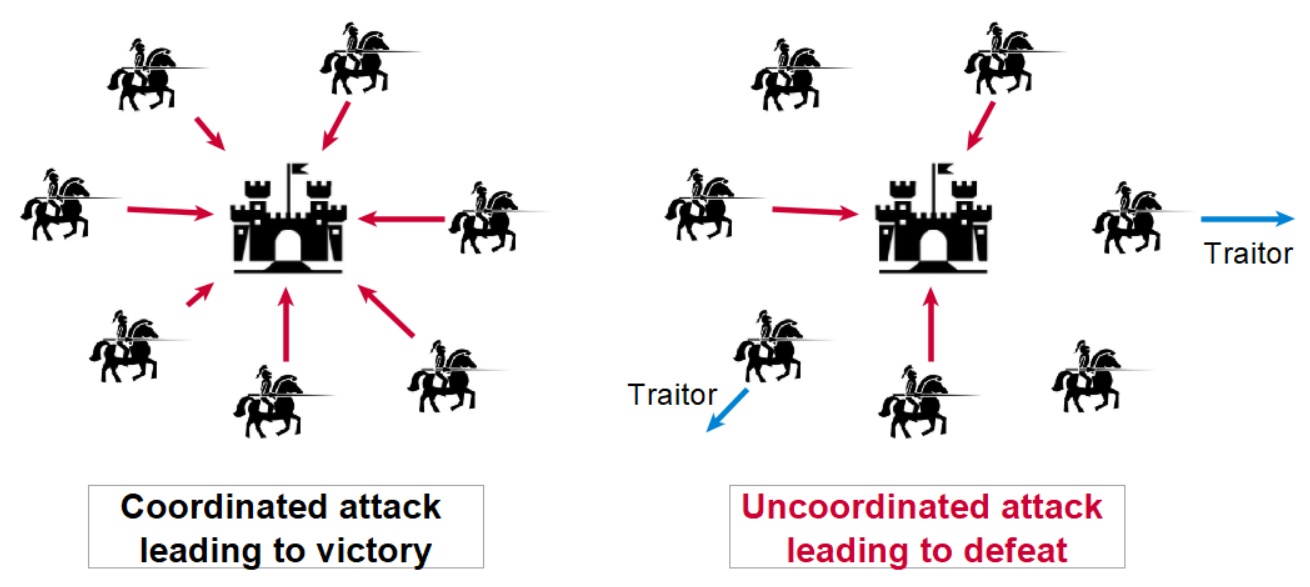
\includegraphics[width=1.0\textwidth]{./immagini/bizantini}
\end{figure}

L'obiettivo da raggiungere è far sì che ai luogotenenti onesti arrivi il piano d’attacco corretto, senza che i traditori possano compromettere l’operazione facendo arrivare loro le informazioni sbagliate.
In una \textit{blockchain}, la soluzione è quella di non avere più un generale che comanda sugli altri. Non c’è più un centro che prevale gerarchicamente, ma si assegna la stessa gerarchia a tutti i partecipanti. Tutti i generali e tutti i luogotenenti, ovvero tutti i nodi, che partecipano a questo modello, concordano ogni singolo messaggio trasmesso, lo vedono e lo condividono. Di conseguenza la \textit{blockchain} è incorruttibile se la maggioranza dei partecipanti risulta essere onesta.


\subsubsection{Algoritmi di consenso}
Gli algoritmi di consenso assicurano la sicurezza e l'integrità dei dati nei sistemi distribuiti. In una \textit{blockchain} l'obiettivo di questi algoritmi è ottenere la validazione delle transazioni, rendere la rete affidabile e prevenire gli attacchi da parte di malintenzionati.
Per ottenere questo risultato i nodi partecipanti devono essere d'accordo sullo stato della \textit{blockchain}. Ogni transazione deve essere registrata nel \textit{ledger} e l’algoritmo di consenso assicura che non ci siano state transazioni maligne o corrotte.
Esistono diversi tipi di algoritmi, ma mi limiterò a spiegare i due principali, su cui si fonda la quasi totalità delle \textit{blockchain}.\\

\paragraph{Proof of work}
L’algoritmo \emph{\gls{proof of work}}\glsfirstoccur si basa sulla generazione di blocchi attraverso complessi problemi matematici, la cui risoluzione richiede un grande sforzo computazionale.
Il meccanismo su cui si basa questo algoritmo è la ricerca di un valore che sottoposto a una funzione \textit{hash} risulti iniziare con un certo numero di zeri. Il lavoro medio è esponenzialmente proporzionale al numero di zeri richiesti. Quello che rende adatto l'\textit{hash} per questo genere di algoritmo è il fatto che sia molto difficile trovare un valore che corrisponda alle caratteristiche richieste, ma estremamente facile verificarne la correttezza.\\ 
Generalmente si adotta un valore \textit{hash} con un numero selezionabile di prime cifre a zero. Il nodo che riesce a trovare il valore \textit{hash} corretto prima degli altri crea il blocco: esso verrà aggiunto in coda alla \textit{blockchain} e riceverà un compenso sotto forma di valuta virtuale, chiamata \emph{\gls{criptovaluta}}\glsfirstoccur.\\ L’algoritmo \textit{proof of work} risolve il problema dei generali bizantini se almeno il 50\% + 1 dei partecipanti alla \textit{blockchain} è onesta: soffre infatti dell'attacco del 51\%.  Se la maggioranza della potenza computazionale della rete fosse controllata da un attaccante o un gruppo di attaccanti, questi avrebbero la possibilità di escludere intenzionalmente transazioni o modificarle a proprio piacimento. Un attacco di questo tipo consentirebbe all'attaccante di invertire le transazioni che ha effettuato, portando a un \emph{\gls{double spending}}\glsfirstoccur. Questo scenario potrebbe fare pensare a gravi problemi di sicurezza nelle \textit{blockchain}, ma in realtà subire un attacco di questo tipo è altamente improbabile, soprattutto nelle \textit{blockchain} di ampia diffusione. Quando una \textit{blockchain} diventa sufficientemente grande, la possibilità che una singola persona o un singolo gruppo di persone sia in grado di controllare il 51\% della rete è quasi nulla.

\paragraph{Proof of stake}
Nel \textit{proof of stake} i blocchi vengono validati da chi possiede più \emph{\gls{token}}\glsfirstoccur nella \textit{blockchain}. Ogni account ha una possibilità proporzionale al proprio saldo di generare un blocco valido. Rispetto al \textit{proof of work}, questo approccio presenta molti vantaggi. Il \textit{proof of work} richiede un'enorme quantità di tempo ed energia e, di conseguenza, un limitato numero di transazioni al secondo e un costo elevato da parte dell’utente per ottenere la validazione della propria transazione. Con il \textit{proof of stake} si ottiene maggiore scalabilità e minor costo per le transazioni.
Inoltre la struttura della \textit{blockchain} la rende più sicura. Se un \textit{miner} detiene la maggioranza dello \textit{stake}, non ha nel suo interesse un attacco alla rete perché se il valore della criptovaluta crolla, crollerebbero anche tutti i suoi averi. Per questo i maggiori proprietari di token hanno nel loro interesse il mantenimento di una rete sicura.

Il \textit{proof of work} è stato il primo algoritmo utilizzato nelle \textit{blockchain} ed è tutt’ora il più diffuso. Negli ultimi anni però stanno nascendo molte \textit{blockchain} che si basano su \textit{proof of stake} e persino \textit{Ethereum}, entro la fine del 2020, inizierà il passaggio al \textit{proof of stake}, che si dovrebbe completare nel 2022.

\subsection{Ethereum}
\textit{Ethereum} è una piattaforma \textit{blockchain} creata nel 2015 da Vitalik Buterik e che ha riscosso fin da subito grande successo.  È nata come alternativa a \textit{Bitcoin}, proponendo la possibilità di eseguire programmi chiamati \textit{smart contract} per creare applicazioni decentralizzate. Anche \textit{Bitcoin} ha un linguaggio che gli permette di creare \textit{smart contract}, ma a differenza della famosa \textit{blockchain}, in \textit{Ethereum} è possibile scrivere contratti \emph{\gls{turing completi}}\glsfirstoccur. Negli \textit{smart contract} è possibile programmare come in qualsiasi altro linguaggio di programmazione, seppur con delle differenze di cui discuteremo più avanti. 


\subsubsection{Smart contract}
Un contratto è un insieme di codice e dati che si trova a uno specifico \textit{address} di \textit{Ethereum}. È un vero e proprio programma che viene eseguito dai nodi della \textit{blockchain}. Gli \textit{smart contract} possono leggere o modificare il proprio stato interno, oltre a mandare o ricevere messaggi e transazioni. Esistono diversi linguaggi che permettono lo sviluppo di \textit{smart contract} in \textit{Ethereum}. I più famosi sono:
\begin{itemize}
	\item{\textit{Solidity}, simile a \textit{JavaScript};}
	\item{\textit{Vyper}: simile a \textit{Python}.}
\end{itemize}
\textit{Solidity} è sicuramente il più diffuso per lo sviluppo di \emph{\gls{applicazioni decentralizzate}}\glsfirstoccur e, per questo motivo, è stato utilizzato durante lo stage.

\subsubsection{Account, transazioni e gas}
\paragraph{Account}\mbox{}\\
In Ethereum ogni partecipante alla blockchain possiede un account con cui interagire nella rete. Anche gli smart contracts hanno un account, fondamentale per raggiungerli e interagire con loro. Gli account hanno un \textit{balance} in \emph{\gls{Ether}}\glsfirstoccur che può essere modificato da transazioni inviate o ricevute.
\paragraph{Transazioni}\mbox{}\\
Una transazione è composta dall'\textit{account target}, l'\textit{account sender}, il valore trasferito in \textit{Ether}, campi dati opzionali, il limite di gas che la transazione può consumare e il prezzo del gas.
\paragraph{Gas}\mbox{}\\
Le transazioni consumano un certo numero di gas, che rappresenta il carburante della blockchain. Ogni operazione negli smart contract ha un costo in gas, detto \emph{\gls{gas price}}\glsfirstoccur, con cui viene calcolato il prezzo della \emph{\gls{fee}}\glsfirstoccur da pagare ai \textit{miner} in \textit{Ether}. Inoltre le operazioni hanno anche un limite di gas, detto \emph{\gls{gas limit}}\glsfirstoccur, ossia la massima quantità di gas che può essere consumata in una transazione. Questo limite protegge la \textit{blockchain} dai \textit{loop} infiniti.

\begin{figure}[!htb]
   \begin{minipage}{0.48\textwidth}
     \centering
     
\includegraphics[width=0.4\textwidth]{./immagini/logo_ethereum}
     \caption{Logo di Ethereum}
   \end{minipage}\hfill
   \begin{minipage}{0.48\textwidth}
     \centering
     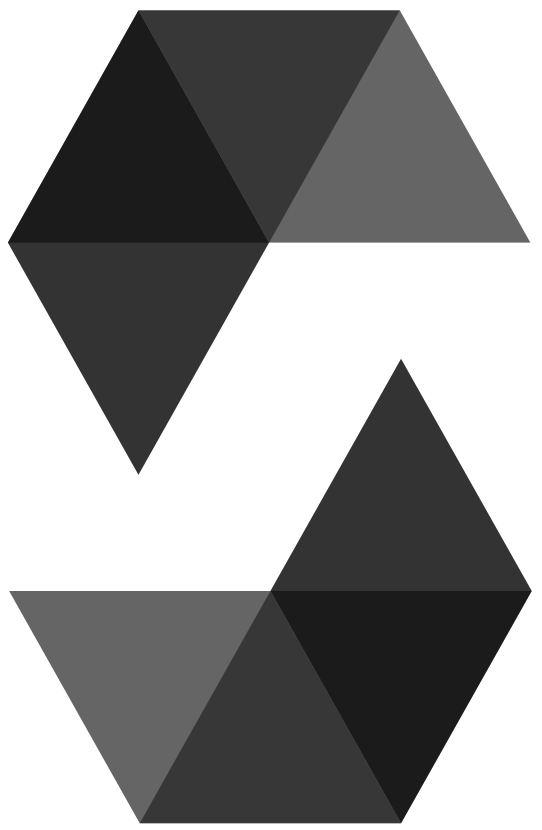
\includegraphics[width=0.425\textwidth]{./immagini/logo_solidity}
     \caption{Logo di Solidity}
   \end{minipage}
\end{figure}

\subsubsection{Solidity}
\textit{Solidity} è un linguaggio tipato che permette di scrivere \textit{smart contract}. I \textit{contratti} a prima vista ricordano molto le classi nella programmazione orientata a oggetti. In \textit{Solidity}, però, bisogna prestare particolare attenzione alla sicurezza, in quanto gli \textit{smart contract} si occupano di gestire transazioni. Se sono presenti bug o falle di sicurezza le conseguenze potrebbero essere gravi. Inoltre è sempre opportuno tenere a mente che le operazioni non sono gratuite, ma vengono pagate con delle \textit{fee} in base al tipo di operazione richiesta. L'efficienza quindi, è cruciale nel definire \textit{smart contract} e non sempre le \emph{\gls{best practices}}\glsfirstoccur in \textit{Solidity} corrispondono alla soluzione che può sembrare migliore in un altro linguaggio di programmazione.

\newpage
Di seguito viene riportato un contratto a titolo esemplificativo:
\begin{lstlisting}[language = Solidity]
pragma solidity ^0.6.8;

contract HelloWorld {

	string hello;
	
	constructor() public {
	    hello = "Hello World!";
	}

	function getHello() public view returns (string memory) {
		return hello;
	}

	function setHello(string memory _hello) public {
		hello = _hello;
	}
}

\end{lstlisting}

\subsubsection{Truffle}
\textit{Truffle} è una suite di supporto per la programmazione in \textit{Solidity} che ha l'obiettivo di rendere la vita dello sviluppatore più semplice. Fornisce un ambiente di sviluppo e un \textit{framework} per testare i contratti usando una \textit{EVM} (\emph{\gls{Ethereum Virtual Machine}}\glsfirstoccur). 
\subsubsection{Web3js e web3j}
Tra gli obiettivi del mio stage c'è l'integrazione dello \textit{smart contract} sviluppato con un ambiente mobile e una web application. Web3.js e web3j servono proprio per raggiungere questo scopo. Sono librerie, la prima per \textit{JavaScript} e la seconda per \textit{Java}, che forniscono il supporto necessario a interagire con il contratto.

%**************************************************************

\section{Analisi dei rischi}

Durante la fase di analisi iniziale, sono stati individuati alcuni rischi che possono essere incontrati durante lo stage. Tali rischi sono riportati di seguito insieme alle loro soluzioni.\\

\begin{risk}{Difficoltà nell'effettuare la maggior parte dello stage in remoto}
    \riskdescription{A causa dell'emergenza sanitaria causata dal COVID-19, gran parte dello stage verrà effettuato da remoto}
    \risksolution{Per affrontare la situazione nel migliore dei modi è opportuno pianificare il lavoro dettagliatamente, avere frequenti aggiornamenti con il tutor aziendale e utilizzare strumenti di supporto}
\end{risk}
\begin{risk}{Scarsa conoscenza delle tecnologie previste per lo svolgimento dello stage}
    \riskdescription{Le \textit{blockchain}, \textit{Ethereum} e lo sviluppo di \textit{smart contract} rappresentano un campo non affrontato durante il percorso di studi e poco conosciuto dal sottoscritto}
    \risksolution{Dedicare molto tempo allo studio approfondito di tutte le tecnologie in gioco per essere preparato a sufficienza al momento dello sviluppo}
\end{risk}
\begin{risk}{Difficoltà nell'integrazione di \textit{Ethereum} con l'ambiente mobile}
    \riskdescription{Il tutor aziendale mi ha avvisato preventivamente della sua scarsa conoscenza in questo ambito e delle possibilti difficoltà che potrebbero emergere}
    \risksolution{In fase di studio tecnologico, dedicare diverse ore ad approfondire questo aspetto}
\end{risk}
\begin{risk}{Tempo limitato per l'integrazione finale con il prodotto sviluppato dall'azienda}
    \riskdescription{Come riportato nel primo rischio, la maggior parte dello stage sarà effettuato da remoto. Il tempo a disposizione con gli altri sviluppatori sarà poco e deve essere sufficiente per portare a termine l'integrazione della \textit{blockchain} nel progetto}
    \risksolution{Ottimizzare il tempo con gli altri sviluppatori in azienda e, se necessario, comunicare con loro organizzando call durante il lavoro svolto da casa}
\end{risk}

%**************************************************************
\section{Vincoli e obiettivi}

\subsection{Vincoli temporali}
Lo stage si svolge in un periodo di 8 settimane lavorative per 8 ore al giorno. Visto il contesto lavorativo da remoto, mi è stato richiesto di compilare quotidianamente un registro delle attività che consentisse al tutor aziendale di verificare il mio lavoro. Verso la fine dello stage mi è stato consentito di lavorare alcuni giorni in azienda, dalle 9:00 alle 18:00. A prescindere dalla modalità di lavoro, ho avuto delle scadenze settimanali da rispettare in base alla pianificazione. 
Infatti, il piano di lavoro presenta un calendario delle attività diviso per settimane che mi ha consentito di tenere sotto controllo lo stato di avanzamento del mio stage.

\subsection{Vincoli metodologici}
Per favorire il lavoro da remoto, il tutor aziendale mi ha fornito un piano delle attività presente su \emph{\gls{Trello}}\glsfirstoccur. Inoltre ogni giorno ho registrato le mie attività in un documento condiviso con il tutor e quasi quotidianamente sono state effettuate call per essere in costante aggiornamento.


\subsection{Vincoli tecnologici}
I vincoli tecnologici che ho dovuto rigorosamente rispettare sono stati:
\begin{itemize}
	\item{Ethereum e Solidity per lo sviluppo dello smart contract;}
	\item{Android per l'integrazione del contract in ambiente mobile;}
	\item{Gitlab per la condivisione del mio lavoro.}
\end{itemize}
Per il resto mi è stata concessa parecchia libertà riguardo agli strumenti di sviluppo e l'uso di tecnologie. Questo ha avuto dei pro e dei contro. Inizialmente ho dovuto dedicare parecchio tempo allo studio ed è stato difficile capire quali fossero le scelte migliori per facilitare il lavoro. A posteriori, però, è stato molto utile e formativo, anche se alcune cose non sono state utilizzate nell'implementazione finale.
\subsection{Obiettivi}
\label{sec:obiettivi}
All'inizio dello stage, il tutor aziendale mi ha posto i seguenti obiettivi da raggiungere entro il termine del percorso:
\begin{center}
	\begin{longtable}{| c | p{30em} |}
		\caption{Tabella degli obiettivi obbligatori}
		\label{tab:obiettivi-obbligatori}\\
		\hline
		\textbf{Obiettivo} & \centering\textbf{Descrizione}\\
		\endfirsthead
		\hline
		\textbf{Obiettivo} & \centering\textbf{Descrizione}\\
		\endhead
		\endfoot
		
		\hline
		O01    & Acquisizione competenze sulle tecnologie blockchain, in particolare Ethereum  \\
		\hline
		O02    & Capacità di progettazione e analisi di smart contract \\
		\hline
		O03    & Capacità di raggiungere gli obiettivi richiesti in autonomia, seguendo il programma preventivato \\
		\hline
		O04    & Portare a termine l'implementazione di almeno l'80\% degli sviluppi previsti \\
		\hline
	\end{longtable}
\end{center}

\begin{center}
	\begin{longtable}{| c | p{30em} |}
		\caption{Tabella degli obiettivi desiderabili}
		\label{tab:obiettivi-desiderabili}\\
		\hline
		\textbf{Obiettivo} & \centering\textbf{Descrizione}\\
		\endfirsthead
		\hline
		\textbf{Obiettivo} & \centering\textbf{Descrizione}\\
		\endhead
		\endfoot
		
		\hline
		D01    & Portare a termine il lavoro di studio della portabilità di Ethereum su dispositivi mobili \\
		\hline
		D02    & Portare a termine l’implementazione completa degli sviluppi previsti \\
		\hline
	\end{longtable}
\end{center}
	
\begin{center}
	\begin{longtable}{| c | p{30em} |}
		\caption{Tabella degli obiettivi facoltativi}
		\label{tab:obiettivi-facoltativi}\\
		\hline
		\textbf{Obiettivo} & \centering\textbf{Descrizione}\\
		\endfirsthead
		\hline
		\textbf{Obiettivo} & \centering\textbf{Descrizione}\\
		\endhead
		\endfoot
		
		\hline
		F01    & Completare l'installazione di un peer su un dispositivo mobile Android \\
		\hline
	\end{longtable}
\end{center}


%**************************************************************
\section{Pianificazione}
Il tutor aziendale ha pianificato il lavoro da svolgere per ogni settimana, nel seguente modo:
\begin{itemize}
        \item \textbf{Prima Settimana (40 ore)}
        \begin{itemize}
            \item Incontro con persone coinvolte nel progetto per discutere i requisiti e le richieste
            relativamente al sistema da sviluppare;
            \item Studio delle diverse tipologie di catene blockhain; 
            \item Studio del funzionamento delle blockchain.
        \end{itemize}
        \item \textbf{Seconda Settimana (40 ore)} 
        \begin{itemize}
            \item Studio di Ethereum, installazione peer e configurazione;
	    \item Ripasso Javascript;	
	    \item Studio linguaggio Solidity.
        \end{itemize}
        \item \textbf{Terza Settimana (40 ore)} 
        \begin{itemize}
            \item Studio linguaggio Solidity.
        \end{itemize}
        \item \textbf{Quarta Settimana (40 ore)} 
        \begin{itemize}
            \item Analisi caso d'uso: creazione smart contract per inserire in catena informazioni sul tracing delle persone;
	    \item Implementazione e testing del codice di smart contract per l'inserimento in catena delle informazioni raccolte sul tracing.
        \end{itemize}
        \item \textbf{Quinta Settimana (40 ore)} 
        \begin{itemize}
            \item Analisi Caso d'uso: creazione smart contract per recuperare da catena le informazioni sul tracing delle persone;
	    \item Implementazione e testing del codice di smart contract per il recupero delle informazioni raccolte sul tracing.
        \end{itemize}
        \item \textbf{Sesta Settimana (40 ore)} 
        \begin{itemize}
            \item Studio Installazione peer Ethereum in ambienti mobile.
        \end{itemize}
        \item \textbf{Settima Settimana (40 ore)} 
        \begin{itemize}
            \item Studio e prototipo di installazione del peer Ethereum in ambienti mobile.
        \end{itemize}
        \item \textbf{Ottava Settimana (40 ore)} 
        \begin{itemize}
            \item Installazioni finali e test;
	    \item Stesura tesina.
        \end{itemize}
    \end{itemize}             % Stage
% !TEX encoding = UTF-8
% !TEX TS-program = pdflatex
% !TEX root = ../tesi.tex

%**************************************************************
\chapter{Analisi dei requisiti}
\label{cap:analisi-requisiti}
%**************************************************************

\intro{In questo capitolo vengono riportati i requisiti richiesti dal prodotto finale con l'utilizzo di una tabella per il tracciamento degli stessi.}\\

\section{Casi d'uso}
All'inizio dello stage sono stati discussi i casi d'uso del software con il tutor aziendale e gli altri stagisti partecipanti al progetto.
L'azienda intende sviluppare un'applicazione mobile per gestire il tracciamento dei contatti e una web application per permettere al personale sanitario di segnalare una persona risultata positiva a un tampone, sempre dietro conferma dell'infetto. Il mio ruolo nel progetto è stato integrare uno smart contract con le due parti. Tuttavia la \textit{blockchain} non è visibile da chi utilizza l'applicazione e non richiede un'interazione con l'utente. I casi d'uso sono stati stilati dai tirocinanti che hanno sviluppato l'applicazione e io mi sono limitato a rispettarli e a trovare i requisiti necessari allo \textit{smart contract} e all'integrazione con il software.
\section{Tracciamento dei requisiti}

Da un'attenta analisi dei requisiti effettuata sul progetto è stata stilata la tabella che traccia i requisiti. Sono stati individuati diversi tipi di requisiti e per distinguerli si è fatto utilizzo di un codice identificativo.\\
Il codice dei requisiti è così strutturato R(F/Q/V)(N/D/O) dove:
\begin{enumerate}
	\item[R =] requisito
    \item[F =] funzionale
    \item[Q =] qualitativo
    \item[V =] di vincolo
    \item[N =] obbligatorio (necessario)
    \item[D =] desiderabile
    \item[Z =] opzionale
\end{enumerate}
Nelle tabelle \ref{tab:requisiti-funzionali}, \ref{tab:requisiti-qualitativi} e \ref{tab:requisiti-vincolo} sono riassunti i requisiti delineati in fase di analisi.

\begin{center}
		\begin{longtable}{| c | p{30em} |}
			\caption{Tabella del tracciamento dei requisiti funzionali}
			\label{tab:requisiti-funzionali}\\
			\hline
			\textbf{Requisito} & \centering\textbf{Descrizione}\\
			\endfirsthead
			\hline
			\textbf{Requisito} & \centering\textbf{Descrizione}\\
			\endhead
			\endfoot
			
			\hline
			RFN-1     & L'address del proprietario del contract deve essere salvato\\
			\hline
			RFN-2     & Una persona deve essere inserita in catena con un id univoco \\
			\hline
			RFN-3     & Un inserimento deve essere rifiutato se è l'id della persona è già presente in catena \\
			\hline
			RFN-4     & Una persona infetta deve essere segnalata in blockchain \\
			\hline
			RFN-5     & Una segnalazione di infezione deve essere rifiutata se non è stata invocata da un medico autorizzato \\
			\hline
			RFN-6     & Una segnalazione di infezione deve essere rifiutata se viene inserito un id non presente in blockchain \\
			\hline
			RFN-7     & Quando viene rilevato un contatto tra due persone deve essere inserito in blockchain\\
			\hline
			RFN-8     & L'inserimento di un contatto viene rifiutato se viene effettuato da un indirizzo non corrispondente a quello della persona il cui contatto viene inserito \\
			\hline
			RFN-9     & L'inserimento di un contatto viene rifiutato se gli id non sono presenti in blockchain \\
			\hline
			RFN-10   & Deve essere possibile ottenere i contatti di una persona negli ultimi 14 giorni \\
			\hline
			RFN-11   & I contatti di una persona non devono essere forniti se vengono richiesti da qualcun altro\\
			\hline
			RFN-12   & Deve essere posssibile stabilire se una persona ha avuto contatti ritenuti a rischio \\
			\hline
			RFN-13   & Un rischio di contagio deve essere confermato anche dai contatti della persona infetta \\
			\hline
			RFN-14   & L'informazione sulla presenza di contatti a rischio deve essere effettuata solo dal proprietario dell'informazione \\
			\hline
			RFN-15   & Deve essere possibile calcolare la somma degli \emph{\gls{indici di contatto}}\glsfirstoccur di una persona negli ultimi gionri\\
			\hline
			RFN-16   & La somma degli indici di contatto deve essere effettuata solo dal proprietario dell'informazione \\
			\hline
			RFN-17   & Deve essere effettuato il deployment dello smart contract \\ 
			\hline
			RFN-18   & Lo smart contract deve essere utilizzato dall'applicazione mobile per l'inserimento dei contatti\\ 
			\hline
			RFN-19   & Lo smart contract deve essere utilizzato dalla web application per l'inserimento degli infetti \\ 
 			\hline
					

		\end{longtable}
	\end{center}

\begin{center}
	\begin{longtable}{| c | p{30em} |}
		\caption{Tabella del tracciamento dei requisiti qualitativi}
		\label{tab:requisiti-qualitativi}\\
		\hline
		\textbf{Requisito} & \centering\textbf{Descrizione}\\
		\endfirsthead
		\hline
		\textbf{Requisito} & \centering\textbf{Descrizione}\\
		\endhead
		\endfoot
		
		\hline
		RQN-1    & Lo smart contract deve essere il più possibile ottimizzato per limitare i consumi di gas \\
		\hline
		RQN-2    & Il codice deve essere versionato e reso disponibile nel \emph{\gls{repository}}\glsfirstoccur aziendale \\
		\hline
		RQN-3    & Deve essere fornito un documento tecnico \\
		\hline
	

	\end{longtable}
\end{center}

\begin{center}
	\begin{longtable}{| c | p{30em} |}
		\caption{Tabella del tracciamento dei requisiti di vincolo}
		\label{tab:requisiti-vincolo}\\
		\hline
		\textbf{Requisito} & \centering\textbf{Descrizione}\\
		\endfirsthead
		\hline
		\textbf{Requisito} & \centering\textbf{Descrizione}\\
		\endhead
		\endfoot
		
		\hline
		RVN-1    & Utilizzo del linguaggio Solidity e piattaforma Ethereum per lo sviluppo dello smart contract  \\
		\hline
		RVD-2    & Installazione dello smart contract in ambiente mobille (Android) \\
		\hline
		RVD-3    & Installazione dello smart contract in ambiente web \\
		\hline			
	\end{longtable}
\end{center}
             % Analisi requisiti
% !TEX encoding = UTF-8
% !TEX TS-program = pdflatex
% !TEX root = ../tesi.tex

%**************************************************************
\chapter{Progettazione e implementazione}
\label{cap:progettazione-codifica}
%**************************************************************

\intro{In questo capitolo viene descritta la progettazione dello smart contract e della sua integrazione nell'applicazione SyncTrace, per poi passare all'implementazione del contratto. Infine si analizza in modo critico lo smart contract dal punto di vista dei consumi, dando possibili alternative di implementazione.}\\

%**************************************************************

\section{Progettazione}
\begin{figure}[h]
\caption{Logo di Synctrace}
\centering

\includegraphics[width=0.5\textwidth]{./immagini/logo_synctrace}
\end{figure}
SyncTrace, il software di \textit{contact tracing} ideato dall'azienda, è formato da due applicativi. Il primo è un'applicazione mobile con cui tracciare i contatti, il secondo è una web application in cui inserire gli infetti.
Lo \textit{smart contract} da sviluppare deve fornire le funzionalità necessarie per entrambi e deve essere possibile utilizzare lo \textit{smart contract} in entrambi gli ambienti.
\subsection{Smart Contract}
Per rispettare i requisiti individuati, si è pensato di utilizzare due strutture, \textit{Person} e \textit{Contact}: \textit{Person} rappresenta una persona, mentre \textit{Contact} è un singolo contatto che una persona ha con un altro utente.\\ Il contratto \textit{Tracing} avrà poi un campo dati di tipo \textit{address} che rappresenta l'indirizzo del proprietario del contratto, una mappa che associa l'id di una persona alla struttura \textit{Person} e una mappa che associa l'id di una persona a un \textit{array} di contatti registrati.
La figura \hyperref[fig:umlcontract]{4.2} riporta un piccolo diagramma riassuntivo che rappresenta lo \textit{smart contract} Tracing, con le varie funzionalità richieste dai requisiti.
\begin{figure}[h]
\label{fig:umlcontract}
\caption{Diagramma \emph{\gls{UML}}\glsfirstoccur smart contract}
\centering
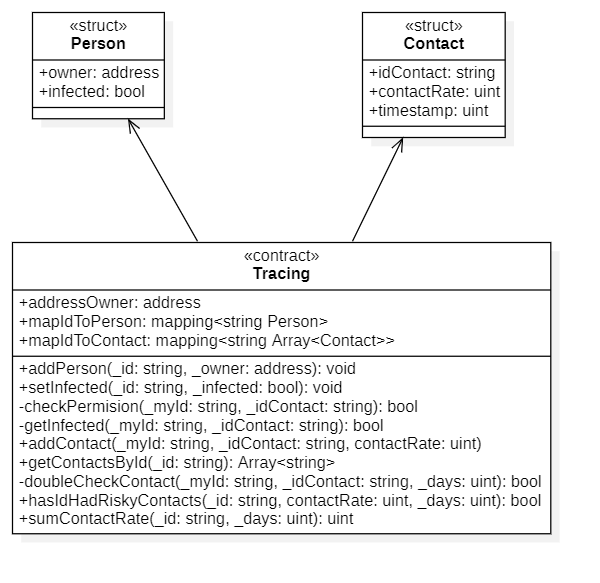
\includegraphics[width=0.75\textwidth]{./immagini/tracingcontractuml}
\end{figure}
\FloatBarrier

Come si può notare dal diagramma, \textit{Person} ha due campi dati:
\begin{itemize}
	\item{\textit{address owner}: indica l'account Ethereum di ogni persona, necessario per permettere l'utilizzo delle funzionalità solo sul proprio account;}
	\item{\textit{bool infected}: booleano che indica lo stato di salute della persona.}
\end{itemize}
Contact invece ha:
\begin{itemize}
	\item{\textit{string idContact}: indica l'id della persona con cui si è entrati in contatto;}
	\item{\textit{uint contactRate}: indica l'indice di contatto avuto, calcolato in base al tempo e alla distanza;}
	\item{\textit{uint timestamp}: indica il momento in cui è stato registrato il contatto.}
\end{itemize}

Una volta effettuato il \emph{\gls{deployment}}\glsfirstoccur, il contratto Tracing deve inizializzare \textit{addressOwner} con l'indirizzo dell'account che ha effettuato il deployment, ossia l'account dell'azienda. Questo account avrà dei privilegi attraverso i quali sarà possibile utillizzare delle funzioni critiche. Per esempio la funzione per segnalare un infetto non deve poter essere chiamata da chiunque, per scongiurare la possibilità che qualcuno possa segnalarsi infetto, anche se non lo è.\\
La mappa che contiene le persone registrate è stata pensata per essere popolata al primo avvio dell'applicazione con un id generato randomicamente.\\
I contatti di ogni persona, invece, saranno aggiunti ogni volta che l'applicazione rileva un contatto tramite la tecnologia bluetooth LE.

\subsection{Integrazione mobile}
Per sfruttare la rete \textit{Ethereum} in android si utilizza la libreria \textit{Java web3j}, nata per lavorare con gli smart contract e interagire con i nodi di \textit{Ethereum}
\begin{figure}[h]
\caption{Integrazione applicazione Java - client Ethereum con web3j}
\centering
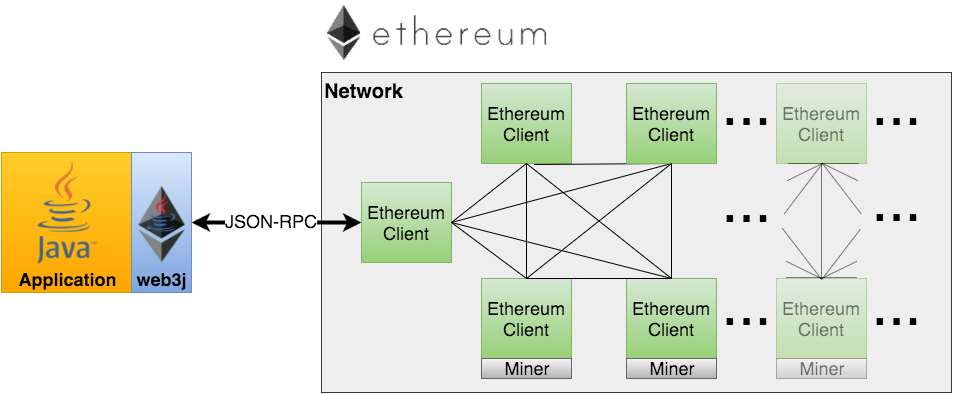
\includegraphics[width=0.8\textwidth]{./immagini/web3j_network.png}
\end{figure}
\FloatBarrier
La figura \hyperref[fig:umlapp]{4.4} riporta un diagramma \textit{uml} che mostra l'integrazione del contratto con l'applicazione mobile SyncTrace.
A partire dal contratto Tracing, grazie a \textit{web3j}, si genera una classe Java \textit{TracingContract} che contiene le funzioni dello \textit{smart contract}, oltre a due metodi per effettuare il \textit{deployment} e il caricamento del contratto.
La classe \textit{TracingContract} viene a sua volta utilizzata da un \textit{BlockchainManager}, che gestisce la configurazione e tutte le operazioni necessarie all'applicazione.
In questo modo, quando nel codice dell'applicazione è necessario effettuare una chiamata allo \textit{smart contract}, è sufficiente instanziare la classe \textit{BlockchainManager} e chiamare il metodo desiderato.
I dettagli relativi all'implementazione nell'applicazione saranno discussi approfonditamente in seguito.

\begin{figure}[h]
\label{fig:umlapp}
\caption{Diagramma di classe integrazione smart contract - SyncTrace app}
\centering
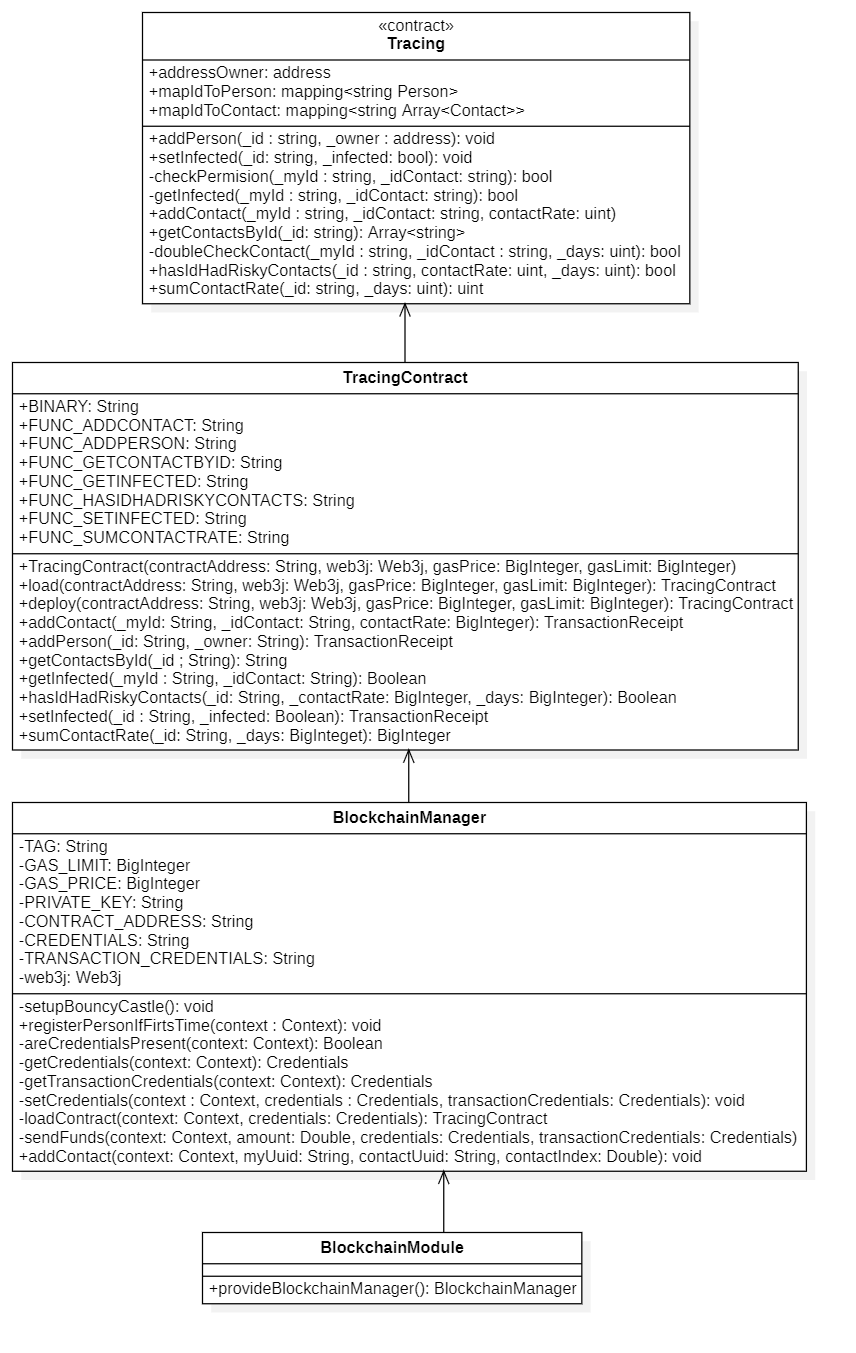
\includegraphics[width=0.76\textwidth]{./immagini/tracinguml.png}
\end{figure}

\FloatBarrier

\subsection{Integrazione web application}
Come nell'ambiente mobile, anche per la web application si utilizza una libreria per interagire con \textit{Ethereum}: \textit{web3js}. 
Per integrare lo \textit{smart contract} alla web app di SyncTrace è sufficiente implementare uno script che configuri la connesione al nodo della \textit{blockchain} e richiami la funzione dello \textit{smart contract} adibita all'inserimento di una persona infetta.
Nel capitolo 5 verrà approfondita la questione.

\subsection{Diagramma di sequenza}
Per comprendere il funzionamento generale di SyncTrace con la \textit{blockchain} riporto un diagramma di sequenza semplificato che mostra come le parti interagiscano nel caso d'uso principale:

\begin{figure}[h]
\caption{Diagramma di sequenza SyncTrace}
\centering
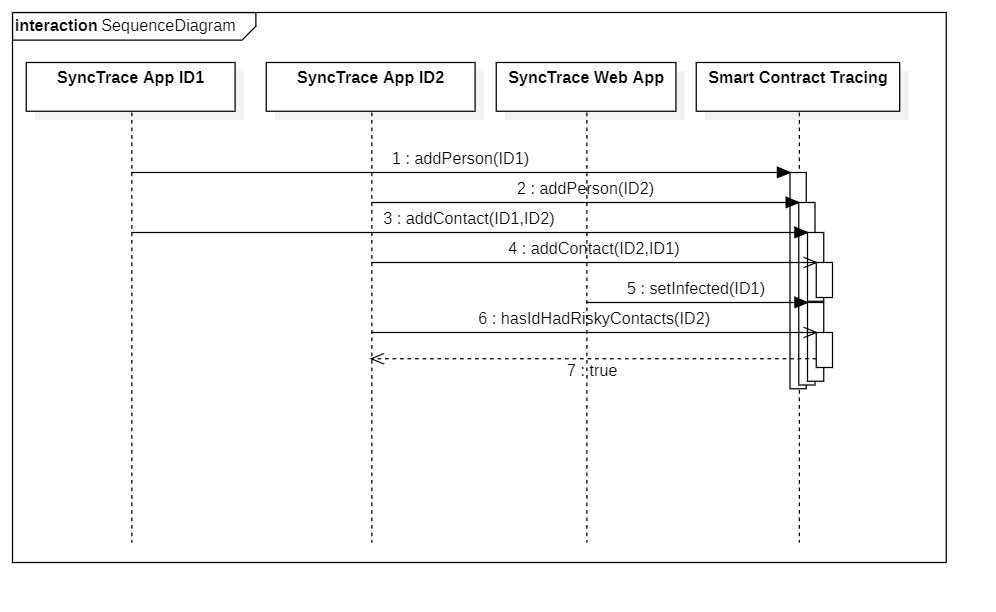
\includegraphics[width=1.0\textwidth]{./immagini/sequenza.png}
\end{figure}

Nel diagramma sono presenti quattro partecipanti: due applicazioni SyncTrace mobile, la web application di SyncTrace e lo \textit{smart contract}.
Quando l'applicazione viene installata negli smartphone, vengono create delle credenziali e l'utente viene aggiunto in catena con il metodo \textit{addPerson}.
Il diagramma, poi, mostra l'aggiunta di un contatto tra le due applicazioni tramite la funzione \textit{addContact}.\\ 
Quando una persona risulta positiva a un tampone, tramite web application, è possibile segnalare il suo stato di salute con la funzione \textit{setInfected}.\\
A questo punto, l'applicazione che ha registrato un contatto con il malato, interrogando la\textit{blockchain} con il suo identificativo, otterrà il valore booleano \textit{true}, che indica che tra i suoi contatti è presente un infetto.


\section{Proof of concept}
Prima di mostrare lo smart contract sviluppato, ritengo utile mostrare una versione inizialmente pensata con il tutor aziendale e implementata come \emph{\gls{Proof of concept}}\glsfirstoccur, per analizzare le differenze tra i due contratti, soprattutto come consumi di gas. Una parte dello stage, infatti, è stata incentrata su come ottimizzare il codice \textit{Solidity}, cercando di progettare lo \textit{smart contract} in modo da raggiungere i requisiti con le operazioni meno onerose nella piattaforma \textit{Ethereum}.
Le funzionalità di questa versione del contratto sono le medesime di quello definitivo e, per questo, non verranno illustrate in questa sezione.
Il codice riportato nelle prossime righe mostra la differenza nelle struct e nei campi dati del contratto rispetto alla progettazione definitiva.

\mbox{\newline}
\begin{lstlisting}[language=Solidity]
pragma solidity ^0.6.7;
pragma experimental ABIEncoderV2;

contract Tracing {

    struct Person {
        string id;
        address owner;
        bool infected;
    }

    struct Contact{
        Person p1;
        Person p2;
        uint256 contactRate;
        uint256 timestamp;
    }

    contract Tracing {
    
        address ownerAddress;
        Person[] people;
        Contact[] contacts;

	/*
		methods
	*/
}

\end{lstlisting}
\mbox{\newline}
Come per la versione definitiva, sono presenti le due struct \textit{Person} e \textit{Contact}, ma con alcune differenze.
\textit{Person} contiene anche l'id dell'utente, mentre \textit{Contact} ha due campi dati \textit{Person} che rappresentano gli utenti entrati in contatto.
Per quanto riguarda i campi dati del contratto, è sempre presente un address con lo stesso scopo, ma il modo di registrare le persone e i contatti è differente. Invece di usare delle mappe sono presenti due \textit{array}, rispettivamente \textit{people} e \textit{contacts}. Lo scopo dell'\textit{array} \textit{people} è sostanzialmente lo stesso della mappa \textit{mapIdToPerson}, ovvero contenere tutti gli utenti registrati. Per registrare i contatti, invece, c'è una grande differenza di progettazione. Invece di associare ogni persona a un'\textit{array} che contenga tutti i contatti che ha, è presente un unico \textit{array contacts}, che include tutti i contatti avuti tra gli utenti.\\
Il \textit{Proof of concept} mostrato è stato scartato per alcune criticità. In primo luogo avere una struttura dati che contenga i contatti di tutti gli utenti non è una soluzione particolarmente furba perché complica inutilmente il contratto in qualsiasi tipo di operazione sui contatti e, soprattutto, perché per il suo funzionamento sono richieste operazioni particolarmente onerose per quanto riguarda il consumo di gas, come il confronto tra stringhe. Infatti in \textit{Solidity} non è supportato il confronto booleano tra due stringhe. Per bypassare questo problema è necessario calcolare l’\textit{hash} delle due stringhe e poi confrontarlo. Il calcolo dell’\textit{hash}, però, è una delle operazioni più onerose in \textit{Ethereum}.\\
Nella sezione \hyperref[sec:gas]{4.3.2} approfondirò l’argomento, mostrando i consumi del \textit{proof of concept} a confronto con il contratto definitivo.

\section{Implementazione}
\subsection{Smart contract Tracing}
L'implementazione dello \textit{smart contract}, come visto nella sezione progettazione, prevede l'utilizzo di due strutture, un address e due mappe per associare l'id di un utente alle sue informazioni e ai suoi contatti.
L'intestazione del contratto, dunque, è la seguente:

\mbox{\newline}
\begin{lstlisting}[language=Solidity]
pragma solidity ^0.6.7;
pragma experimental ABIEncoderV2;

contract Tracing {

    struct Person {
        address owner;
        bool infected;
    }

    struct Contact {
        bytes32 idContact;
        uint256 contactRate;
        uint256 timestamp;
    }
    
    address ownerAddress;
    mapping(bytes32 => Person) mapIdToPerson;
    mapping(bytes32 => Contact[]) mapIdToContact;

	/*
	methods
	*/
}

\end{lstlisting}
È disponibile un costruttore che al momento del \textit{deployment} assegna la variabile \textit{addresOwner} al chiamante \textit{msg.sender}:

\mbox{\newline}
\begin{lstlisting}[language = Solidity]

    constructor() public {
        ownerContract = msg.sender;
    }

\end{lstlisting}
\mbox{\newline}

Inoltre viene dichiarato un modificatore che viene utilizzato da diverse funzioni del contratto.
In \textit{Solidity} un modificatore viene eseguito prima della funzione in cui ne viene richiesto l'utilizzo. Come un metodo, ha un nome e degli argomenti, e al suo interno si trova una condizione. Se la condizione è soddisfatta, viene eseguito il corpo della funzione che utilizza il modificatore; in caso contrario la funzione non viene eseguita.\\
Nel \textit{contract Tracing} la condizione del modificatore \textit{isOwner} è di eseguire la funzione se e solo se l'utente che chiama il metodo ha l'address che corrisponde a quello salvato nel campo dati \textit{owner} della persona con id dato in input. In questo modo le funzioni in cui viene specificata questa condizione possono essere eseguite solo da chi ha i permessi per farlo. Il modificatore è il seguente:

\mbox{\newline}
\begin{lstlisting}[language = Solidity]

    modifier isOwner(bytes32 _id) { 
        require(msg.sender == mapIdToPerson[_id].owner,"You are not the owner");
        _; 
    }

\end{lstlisting}
\mbox{\newline}

Sono state implementate delle funzioni ad uso interno, ossia non visibili e non eseguibili se non all'interno dello \textit{smart contract}.
Sono funzioni di utilità utilizzate da alcuni metodi pubblici e per questo non sono disponibili all'utente:

\mbox{\newline}
\begin{lstlisting}[language = Solidity]

/*
Funzione di utilita' che prende in input l'id di chi chiama la funzione e l'id del contatto da verificare.
Prima dell'esecuzione chiama il modificatore isOwner per verificare i permessi.
Ritorna il valore del booleano infected per la persona di id = _idContact
*/
function getInfected(bytes32 _myId,bytes32 _idContact) internal view isOwner(_myId) returns (bool);

/*
Funzione di utilita' che prende in input l'id di chiama la funzione, l'id del contatto da verificare e il numero dei giorni da controllare.
Verifica che se il primo id ha aviuto un contatto con il secondo id, anche il secondo id deve aver avuto un contatto con il primo.
Ritorna un booleano che indica il risultato del controllo
*/
function doubleCheckContact(bytes32 _myId, bytes32 _idContact,uint _days) internal view returns (bool);

\end{lstlisting}
\mbox{\newline}

Infine le funzioni disponibili all'utente hanno tutte come visibilità \textit{external} e sono le seguenti:

\mbox{\newline}
\begin{lstlisting}[language=Solidity]
/*
Funzione che prende in input l'id e l'indirizzo di una persona e l'aggiunge alla mappa mapIdToPerson.
Se la persona e' gia' presente nella mappa, viene restituito un errore.
*/
function addPerson(bytes32 _id, address _owner) external;

/*
Funzione che prende in input l'id di una persona e un booleano che indica il suo stato di salute (infetto o meno). e cambia la variabile infected della persona con l'id inserito. 
Puo' essere chiamata solo dall'account proprietario del contratto (chi ha fatto il deployment)
Restituisce un errore se l'id non e' registrato.
*/    
function setInfected(bytes32 _id,bool _infected) external;

/*
Funzione che prende in input l'id del chiamante, l'id del contatto avuto e un indice di contatto.
Aggiunge un contatto con i dati in input alla mappa mapIdToContacts.
Restituisce un errore se il chiamante non ha i permessi per inserire il contatto o se gli id inseriti non sono registrati.
*/    
function addContact(bytes32 _myId,bytes32 _idContact,uint _contactRate) external isOwner(_myId);

/*
Funzione che prende in input un id e restituisce un array contenente i contatti dell'id inserito.
Restituisce un errore se il chiamante non ha i permessi per richiedere i contatti oppure se l'id inserito non e' registrato.
*/    
function getContactsById(bytes32 _id) external view isOwner(_id) returns(bytes32[] memory);

/*
Funzione che prende in input un id, un indice di contatto e un numero di giorni.
Controlla se tra i contatti della persona con l'id inserito ci sia un contatto con una persona infetta.
Il contatto deve avere indice superiore a quello indicato e deve essere avvenuto negli ultimi giorni inseriti in input.
Restituisce un errore se il chiamante non ha i permessi necessari.
*/    
function hasIdHadRiskyContacts(bytes32 _id,uint _contactRate,uint _days) external view isOwner(_id) returns (bool);

\end{lstlisting}
\newpage
\begin{lstlisting}[language=Solidity]
/*
Funzione che prende in indice un id e un numero di giorni.
Ritorna la somma degli indici di contatto per l'id in input negli ultimi giorni indicati.
Restituisce un errore se il chiamante non ha i permessi necessari.
*/   
function sumContactRate(bytes32 _id,uint256 _days) external view isOwner(_id) returns (uint256);

\end{lstlisting}

\mbox{\newline}

\subsection{Analisi gas}
\label{sec:gas}
In \textit{Ethereum} ogni operazione effettuata, che cambia lo stato della \textit{blockchain}, consuma gas. Il gas è un’unità di misura utilizzata per pagare la computazione effettuata dai \textit{miner}. Più un'operazione è dispendiosa a livello di risorse, più gas questa operazione costa.
Il concetto di gas permette di addebitare una tariffa che viene pagata ai \textit{miner}, incentivandoli a prendere parte attiva al sistema.\\
Tuttavia, il gas rappresenta un cambio di paradigma rispetto alla programmazione classica. Non sempre un approccio vantaggioso in un normale linguaggio di programmazione rappresenta la \textit{best practice} in \textit{Solidity}, proprio perché c’è una variabile in più da considerare. 
Nel corso dello stage è stata rivolta particolare attenzione a questo aspetto: il \textit{contract} è stato ottimizzato per cercare di limitare il più possibile il consumo di gas.\\

Dal \textit{Proof of concept} allo \textit{smart contract} finale, infatti, la differenza di gas per il \textit{deployment} e per le operazioni è notevole. Nelle tabelle successive sono riporatati i consumi per entrambe le versioni. I costi stimati in euro fanno riferimento all'attuale tasso di conversione di 202 euro/ether. Il costo per unità di gas, invece è 26 \emph{\gls{gwei}}\glsfirstoccur/gas.
\newpage
\begin{center}
	\begin{longtable}{| c | c | c |}
		\caption{Tabella gas Proof of Concept}
		\label{tab:gas-poc}\\
		\hline
		\textbf{Metodo} & \textbf{Consumo gas medio} & \textbf{Costo medio (eur)}\\
		\endfirsthead
		\hline
		\textbf{Metodo} & \textbf{Consumo gas medio} & \textbf{Costo medio (eur)}\\
		\endhead
		\textbf{Deployment} & \textbf{1599579} & \textbf{8.41}\\
		\hline
		\endfoot
		
		\hline
		addPerson & 79367 & 0.41\\
		\hline
		addContact & 203512 & 1.07\\
		\hline
		setInfected & 50111 & 0.26\\
		\hline
	\end{longtable}
\end{center}

\begin{center}
	\begin{longtable}{| c | c | c |}
		\caption{Tabella gas Tracing}
		\label{tab:gas-tracing}\\
		\hline
		\textbf{Metodo} & \textbf{Consumo gas medio} & \textbf{Costo medio (eur)}\\
		\endfirsthead
		\hline
		\textbf{Metodo} & \textbf{Consumo gas medio} & \textbf{Costo medio (eur)}\\
		\endhead
		\textbf{Deployment} & \textbf{839416} & \textbf{4.41}\\
		\hline
		\endfoot
		
		\hline
		addPerson & 43859 & 0.23\\
		\hline
		addContact & 104806 & 0.55\\
		\hline
		setInfected & 29364 & 0.15\\
		\hline
	\end{longtable}
\end{center}

Come si può notare, il costo del \textit{deployment} dei due \textit{smart contract} è quasi dimezzato: 1.600.000 contro 830.000. Il risparmio c'è, ma non è il più significativo pensando al fatto che il \textit{deployment} viene effettuato una singola volta. Il costo del \textit{deployment}, in un'applicazione \textit{Ethereum}, è abbastanza marginale rispetto al costo delle operazioni se, come in questo caso, le funzioni devono essere chiamate molte volte.
Risulta molto più interessante analizzare il consumo delle funzioni \textit{addPerson}, \textit{addContact} e \textit{setInfected}. Anche per queste operazioni il risparmio è molto importante: ogni chiamata ha un consumo all'incirca dimezzato rispetto al \textit{Proof of Concept}:
\begin{itemize}
\item{\textit{addPerson}: 79367 prima, 43859 dopo}
\item{\textit{addContact}: 203512 prima, 104806 dopo}
\item{\textit{setInfected}: 50111 prima, 29364 dopo}
\end{itemize}

Questi risultati sono in parte dovuti alla modifica progettuale del contratto. Nel \textit{Proof of Concept} sono stati utilizzati \textit{array} dinamici per contenere gli utenti registrati e i contatti. Al contrario, nello \textit{smart contract} finale, si è fatto uso di mappe. In \textit{Solidity} gli array dinamici hanno delle \textit{features} che li rendono inevitabilmente più costosi come: 
\begin{itemize}
\item{La variabile \textit{length}, per contare il numero di oggetti memorizzati;}
\item{Il \textit{bound-checking} per avere un controllo sull'accesso casuale.}
\end{itemize}

Inoltre, grazie all'utilizzo delle mappe, le funzioni dello \textit{smart contract} risultano essere più semplici e con meno operazioni da effettuare. Un esempio lampante è il confronto tra stringhe. Per la natura del contratto, nel \textit{Proof of concept} è necessario confrontare più volte gli id di tipo stringa. Il confronto booleano tra stringhe, però, non esiste in \textit{Solidity}. Si può risolvere questa problematica calcolando l'\textit{hash} delle stringhe, per poi confrontare il risultato. Tuttavia, l'operazione di \textit{hashing} è una tra le più onerose e aumenta sensibilmente il costo del contratto.\\

Sono stati presi altri accorgimenti per il risparmio di gas come:
\begin{itemize}
\item{\textbf{Funzioni interne: }è stata utilizzzata la visibilità internal per le funzioni non utilizzate all'esterno del contratto;}
\item{\textbf{Funzioni esterne: }è stata utilizzata la visibilità external invece di quella public;}
\item{\textbf{Storage: }sono state limitate le operazioni di storage;}
\item{\textbf{Eventi: }gli eventi non sono stati utilizzati. Le funzioni che emettono eventi hanno un costo molto superiore;}
\item{\textbf{Tipo bytes: }dove possibile è stato utilizzato il tipo bytes invece del tipo stringa;}
\item{\textbf{Assert vs require: }le eccezioni sono state gestite con la keyword require;}
\item{\textbf{Ottimizzazione compilazione: }la compilazione Solidity è stata ottimizzata con la keyword optimize;}
\end{itemize}

\subsection{Fattibilità applicazione reale}
Anche con la massima efficienza di uno smart contract, è fondamentale considerare il caso d’uso dell’applicazione, per rendersi conto della fattibilità del progetto.
Come accennato prima, i costi maggiori in \textit{Ethereum} non sono rappresentati dal \textit{deployment} del contratto, bensì dal numero di chiamate stimate alle funzioni che consumano gas.
Nel nostro caso d’uso, la funzione \textit{addPerson} viene eseguita ogni qualvolta una persona installa l’applicazione nel proprio smartphone. Considerando come campione metà della popolazione italiana, il metodo viene chiamato 30 milioni di volte. Con il prezzo attuale dell'\textit{Ether} (202 euro/Ether) e impostando il \textit{gas price} a 26 gwei/gas, ogni chiamata costa circa 23 centesimi. Questo vuol dire che solo per l’installazione il costo stimato è di 7,5 milioni di euro.
Già questo piccolo calcolo sarebbe sufficiente per rendersi conto che questo \textit{smart contract} non è sostenibile in un contesto di utilizzo reale. Purtroppo però, c’è una spesa ancora maggiore. In \textit{blockchain} viene inserito ogni contatto superiore a 15 minuti, a distanza inferiore di 2 metri, per ogni persona che ha l’applicazione. Con il \textit{gas price} e il tasso di cambio indicati, la chiamata per aggiungere un contatto ha un costo di circa 50 centesimi e non è difficile immaginare che il numero di chiamate sia di svariati milioni al giorno. Per questo motivo, soluzioni di questo genere sono difficilmente utilizzabili nella realtà.
Tuttavia ci sono delle soluzioni alternative.
\\
\subsection{Soluzioni}
\subsubsection{Smart contract semplificato}
Come detto, in \textit{Ethereum}, la soluzione proposta non è realizzabile nella pratica. Una possibile alternativa nell’ambito contact tracing è rappresentata dalla gestione locale di tutti i contatti tra le persone. Ogni dispositivo mobile possiede un id; i contatti con gli altri dispositivi vengono registrati e salvati localmente. Ogni 14 giorni vengono eliminati perché considerati ininfluenti per il contagio.
Quando una persona viene trovata infetta a seguito di un tampone, il medico (sotto autorizzazione del contagiato) lo segnala tramite web app. A seguito di questa segnalazione, l’id del malato viene inserito nell’\textit{array} degli infetti nello \textit{smart contract}. 
In questo modo lo \textit{smart contract} risulta estremamente più semplice. Gestisce un \textit{array} di infetti con una funzione per l'aggiunta e una per la rimozione, in modo sicuro e immutabile.
Lo smart contract in questione potrebbe essere implementato in questo modo:

\mbox{\newline}
\begin{lstlisting}[language = Solidity]
pragma solidity ^0.6.7;
pragma experimental ABIEncoderV2;

contract Tracing {

    bytes32[] infected;
    
    function addInfected(bytes32 _id) external {
        //require only doctors
        infected.push(_id);
    }

    function removeInfected(bytes32 _id) external {
        //require only doctors
        for(uint i = 0; i < infected.length; i++) {
            if(infected[i] == _id) {
                infected[i] = infected[infected.length - 1];
                infected.pop();
            }
        }
    }  
    
    function getInfected() external view returns (bytes32[] memory){   
        uint length = 0;
        for(uint i = infected.length; i > 0; i--) {
            length++;
        }
        bytes32[] memory toReturn = new bytes32[](length);
        for(uint i = infected.length; i > 0; i--) {
            toReturn[i-1] = infected[i-1]; 
        }
        return toReturn;
    }
   
}
\end{lstlisting}
\mbox{\newline}

Lato mobile, periodicamente il dispositivo chiama la funzione dello \textit{smart contract} che restituisce gli infetti. Gli id ritornati vengono confrontati con gli id dei contatti salvati localmente per verificare la presenza di un rischio contagio.
Tutte le altre operazioni sono effettuate localmente. Il consumo del gas è infinitamente più contenuto e permette un utilizzo reale dell’applicazione. Questo perché le uniche operazione che richiedono una transazione, e dunque un consumo di gas, sono quelle di inserimento e rimozione di un id nell’\textit{array}. Questi metodi possono essere eseguiti solo dal personale sanitario a seguito di un tampone risultato positivo. \\
Il consumo di gas per questo \textit{smart contract} è riportato nella seguente tabella:
\begin{center}
	\begin{longtable}{| c | c | c |}
		\caption{Tabella gas smart contract semplificato}
		\label{tab:gas-simplytracing}\\
		\hline
		\textbf{Metodo} & \textbf{Consumo gas medio} & \textbf{Costo medio (eur)}\\
		\endfirsthead
		\hline
		\textbf{Metodo} & \textbf{Consumo gas medio} & \textbf{Costo medio (eur)}\\
		\endhead
		\textbf{Deployment} & \textbf{196237} & \textbf{1.04}\\
		\hline
		\endfoot
		
		\hline
		addInfected & 52272 & 0.28\\
		\hline
		removeInfected & 28353 & 0.15\\
		\hline
	\end{longtable}
\end{center}

Dalla tabella si può notare come il costo di \textit{deployment} del contratto sia notevolmente inferiore rispetto al precedente: 1.500.000 gas contro 200.000 circa. 
Ma la differenza la fa soprattutto il numero di chiamate alle funzioni \textit{addInfected} e \textit{removeInfected}, decisamente inferiori rispetto a tutte le chiamate necessarie per registrare i contatti.
In Italia i contagi certificati ad oggi sono circa 200 mila. Considerando un costo di circa 20 centesimi a chiamata per ogni infetto, supponendo anche che tutti gli infetti siano registrati all’applicazione e diano il consenso al proprio medico, la spesa totale dell’utilizzo del contratto si aggirerebbe intorno a 40 mila euro, in linea con le \textit{dApp} più utilizzate. \\
\subsubsection{Altre blockchain}
Un’altra soluzione, che può essere anche complementare a quella appena descritta, prevede un cambio di piattaforma. \textit{Ethereum} infatti, nonostante sia la \textit{blockchain} più diffusa per lo sviluppo di \textit{applicazioni decentralizzate}, ha un costo molto alto e destinato ad aumentare con l’aumentare degli utenti.
Questo è dovuto all’algoritmo di consenso che \textit{Ethereum}, come la maggiorparte delle \textit{blockchain}, utilizza attualmente, ossia il \textit{proof of work}. La computazione richiesta per validare i blocchi e le transazioni richiedono il pagamento di una \textit{fee}, proporzionale alle risorse richieste. 
Tuttavia, esistono altri tipi di \textit{blockchain} che utilizzano il consenso \textit{proof of stake}, come la piattaforma EOS.
La scalabilità e le transazioni gratuite sono i punti di forza di EOS. Il processo non è comunque gratuito, ma richiede che l’utente possieda un numero di \textit{token (stake)} che gli permetta di “affittare” le risorse necessarie per validare le transazioni. Questi \textit{token}, però, non sono spesi, ma possono essere restituiti quando desiderato al prezzo corrente della criptovaluta.
Anche \textit{Ethereum} sta effettuando il passaggio al \textit{proof of stake}, con la piattaforma che verrà denominata \textit{Ethereum 2.0}, in arrivo a fine 2020. 
Il passaggio definitivo, con la chiusura di \textit{Ethereum 1.0} è previsto per il 2022.
\textit{Ethereum 2.0} è molto atteso perché il \textit{proof of stake} cambia completamente il modo di vedere le \textit{blockchain}. La scalabilità è uno dei problemi maggiori delle \textit{blockchain} che si basano su \textit{proof of work}, limitandone possibili applicazioni. Con \textit{Ethereum 2.0}, invece, potrebbe essere possibile utilizzare le \textit{blockchain} per qualsiasi tipo di \textit{applicazione decentralizzata}, senza accusare differenze rispetto a quelle tradizionali.

\section{Test smart contract}
I test dello \textit{smart contract} sono stati fatti con il linguaggio JavaScript sfruttando la \textit{suite truffle}.
Di seguito è riportata la tabella di tracciamento dei test.

\begin{center}
	\begin{longtable}{| c | p{25em} | c |}
		\caption{Tabella test smart contracti}
		\label{tab:test-sci}\\
		\hline
		\textbf{Test id} & \centering\textbf{Descrizione} & \textbf{Requisiti coperti}\\
		\endfirsthead
		\hline
		\textbf{Test id} & \centering\textbf{Descrizione} & \textbf{Requisiti coperti}\\
		\endhead
		\endfoot
		
		\hline
		UT-1     & Should deploy smart contract properly and save owner address & RFN-1 \\
		\hline
		UT-2     & Should add two person to people array and get them by id & RFN-2 - RF10\\
		\hline
		UT-3     & Should not be able to add the same id person in people array & RFN-3 \\
		\hline
		UT-4     & Should add a contact between two id presents in people array & RFN-7 \\
		\hline
		UT-5     & Should not be able to add another person contacts & RFN-8 \\
		\hline
		UT-6     & Should not be able to add a contact with nonexisting person & RFN-9 \\
		\hline
		UT-7     & Should set a person infected & RFN-4 \\
		\hline
		UT-8     & Should not be able to set a person infected if the address is not who deploys the contract & RFN-5 \\
		\hline
		UT-9     & Should not be able to set infected a nonexisting person & RFN-6 \\
		\hline
		UT-10   & Should not be able to get other people contacts & RFN-11 \\
		\hline
		UT-11   & Should check that the second id has a infection risk & RFN-12 \\
		\hline
		UT-12   & Should check that if a contact is not confirmed, then a person has not risk infection &  13\\
		\hline
		UT-13   & Should not be able to check another person risk infection & RFN-14 \\
		\hline
		UT-14   & Should check that sum of contactRates in the last day is 15 for the first id & RFN-15 \\
		\hline
		UT-15   & Should not be able to calculate another person sum of contactRates & RFN-16 \\
		\hline
	\end{longtable}
\end{center}
             % Progettazione e implementazione
% !TEX encoding = UTF-8
% !TEX TS-program = pdflatex
% !TEX root = ../tesi.tex

%**************************************************************
\chapter{Integrazione in SyncTrace}
\label{cap:integrazione-synctrace}
\intro{In questo capitolo viene mostrata l'integrazione dello smart contract con l'applicazione mobile e la web application di SyncTrace.}\\

\section{Applicazione android}
\begin{figure}[!htb]
   \begin{minipage}{0.48\textwidth}
     \centering
     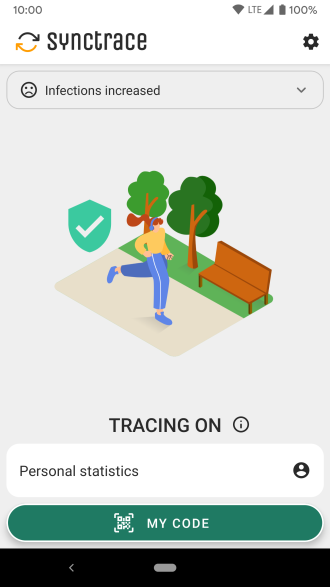
\includegraphics[width=0.65\textwidth]{./immagini/appnormal}
     \caption{Schermata principale SyncTrace senza rischio contagio}
   \end{minipage}\hfill
   \begin{minipage}{0.48\textwidth}
     \centering
     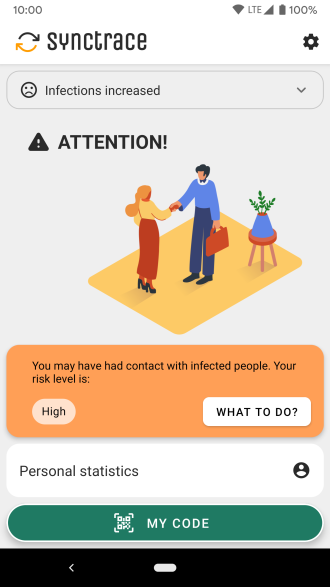
\includegraphics[width=0.65\textwidth]{./immagini/appinfection}
     \caption{Schermata principale SyncTrace con rischio contagio}
   \end{minipage}
\end{figure}
\FloatBarrier
\subsection{Obiettivo}
L'obiettivo dell'integrazione con l'applicazione è implementare una classe che gestisca il contratto e tutte le operazioni legate alla \textit{blockchain}, come visto in fase di progettazione. In particolare è necessario avere a disposizione:
\begin{itemize}
	\item{Credenziali per ogni utente da creare al primo avvio dell'app;}
	\item{Trasferimento di \textit{Ether} a ogni utente, con ricarica all'esaurimento;}
	\item{Gestione delle funzioni dello \textit{smart contract} richieste dall'applicazione, come l'aggiunta dei contatti.}
\end{itemize}

\subsection{Generazione classe Tracing.java}
Per potere utilizzare lo \textit{smart contract}, bisogna generare una classe Java a partire dal contratto, sfruttando \textit{web3j}. La classe generata renderà disponibili i metodi dello \textit{smart contract}, oltre a funzioni per effettuare il \textit{deployment} e caricare un contratto.\\\\
La prima cosa da fare è scaricare \textit{web3j} dalla repo su \href{https://github.com/web3j/web3j/releases}{Github} ed estrarre il file zip scaricato con il comando:
\begin{lstlisting}[numbers=none]
	unzip web3j-<version>.zip
\end{lstlisting}
Sempre da terminale, si può avviare web3j in questo modo:
\begin{lstlisting}[numbers=none]
	web3j-<version>/bin/web3j
\end{lstlisting}
A questo punto è possibile creare i file .abi e .bin dello smart contract con il comando: 
\begin{lstlisting}[numbers=none]
	solcjs ./Tracing.sol --bin --abi --optimize -o ./ 
\end{lstlisting}
A partire dai file .bin e .abi si può finalmente generare la classe java:
\begin{lstlisting}[numbers=none]
	web3j solidity generate -b ./Tracing.bin -a ./Tracing.abi -o ./ -p GeneratedClasses 
\end{lstlisting}
In questo modo nella directory GeneratedClasses si troverà la classe Tracing.java, da inserire nel progetto di android per permettere l'integrazione dell'app con la blockchain.
L'ultimo passaggio da effettuare per interagire con il contract è includere nel file build.gradle del progetto la dipendenza con la libreria web3j, inserendo la seguente riga:
\begin{lstlisting}[numbers=none]
	implementation'org.web3j:core:<version>' 
\end{lstlisting}

\subsection{Implementazione}
Oltre alla classe \textit{Tracing.java}, generata da \textit{web3j}, è necessario implementare una classe che si occupi di configurare e gestire le operazioni in \textit{blockchain}.
Nel progetto SyncTrace è stata creata la classe \textit{BlockchainManager} per questo scopo, scritta in linguaggio Kotlin come il resto dell'applicazione.
Per configurare correttamente il collegamento con lo \textit{smart contract} sono necessarie le seguenti variabili:
\begin{lstlisting}[language = Kotlin]
    private val GAS_LIMIT = BigInteger.valueOf(GAS_LIMIT)
    private val GAS_PRICE = BigInteger.valueOf(GAS_PRICE)
    private const val PRIVATE_KEY = YOUR_PRIVATE_KEY
    private const val CONTRACT_ADDRESS = ADDRESS
    private const val CREDENTIALS = "bc_credentials"
    private const val TRANSACTION_CREDENTIALS = "bc_transaction_credentials"
    private val web3j = Web3j.build(HttpService(
        "https://ropsten.infura.io/v3/YOUR_INFURA_ID"
    ))
\end{lstlisting}
\mbox{\\}

\textit{GAS\_LIMIT} e \textit{GAS\_PRICE} sono i valori relativi al gas in \textit{Ethereum} e devono essere passati nelle funzioni che richiedono una transazione.\\\\
La variabile \textit{PRIVATE\_KEY} è la chiave privata dell'account \emph{\gls{Metamask}}\glsfirstoccur che finanzia l'applicazione.\\\\
\textit{CONTRACT\_ADDRESS} è l'indirizzo del contratto nella \textit{blockchain}. È possibile effettuare il \textit{deployment} anche tramite \textit{web3j} e ottenere l'\textit{address} del contratto da utilizzare.\\\\
\textit{CREDENTIALS} e \textit{TRANSACTION\_CREDENTIALS} rappresentano le keyword utilizzate per salvare le credenziali nelle \textit{shared preferences} di android. Vengono create al primo avvio dell'app e salvate per essere utilizzate nel chiamare le funzioni dello \textit{smart contract}.\\\\ 
\textit{web3j} è un'istanza utilizzata per fornire un client eseguito tramite il provider Infura.\\\\

\newpage
Nella classe sono disponibili alcune funzioni di utilità utilizzate dai metodi che verranno successivamente descritti:
\begin{lstlisting}[language = Kotlin]

/*
Controlla se le credenziali siano gia' state salvate nelle shared preferences
*/
private fun areCredentialsPresent(context: Context): Boolean


/*
Ritorna le credenziali dell'utente dalle shared preferences
*/
private fun getCredentials(context: Context): Credentials

/*
Ritorna le credenziali dell'admin dalle shared preferences
*/
private fun getTransactionCredentials(context: Context): Credentials

/*
Salva le credenziali nelle shared preferences
*/
private fun setCredentials(context: Context, credentials: Credentials,
                               transactionCredentials: Credentials)

/*
Ritorna un'istanza del contratto
*/
private fun loadContract(context: Context, credentials: Credentials = getCredentials(context)): TracingContract

/*
Effettua una transazione dall'account admin all'account utente
*/
private fun sendFunds(context: Context, amount: Double,
                          credentials: Credentials = getCredentials(context),
                          transactionCredentials: Credentials = getTransactionCredentials(context))
\end{lstlisting} 

\newpage
Al primo avvio dell'applicazione bisogna creare delle credenziali per il nuovo account, effettuare una transazione verso questo account, caricare il contratto \textit{Tracing} e infine aggiungere l'utente in \textit{blockchain} tramite la funzione \textit{addPerson} dello \textit{smart contract}. La funzione \textit{registerPersonIfFirstTime} si occupa di tutto ciò
\begin{lstlisting}[language = Kotlin]
    fun registerPersonIfFirstTime(context: Context) {
        if (!areCredentialsPresent(context)) {
            val transactionCredentials = Credentials.create(PRIVATE_KEY)
            // create new private/public key pair
            val keys = Keys.createEcKeyPair()
            val uuid = User.getUuid(context)
            val wallet = Wallet.createLight(uuid, keys)
            val credentials = Credentials.create(Wallet.decrypt(uuid, wallet))

            sendFunds(context, 0.2, credentials, transactionCredentials)

            try {
                val tracingContract = loadContract(context, credentials)
                tracingContract.addPerson(uuid, credentials.address).sendAsync().get()
            } catch (e: Exception) {
                Log.e(TAG, "Cannot add person", e)
                return
            }

            setCredentials(context, credentials, transactionCredentials)
            Log.i(TAG, "Created credentials and registered person")
        }
    }
\end{lstlisting}

\newpage
Infine la classe \textit{BlockchainManager} deve fornire una funzione per ogni metodo del contratto che viene utilizzato nell'applicazione, come per il metodo \textit{addContact} che aggiunge un contatto in \textit{blockchain} quando rilevato dal bluetooth.

\mbox{\\}
\begin{lstlisting}[language = Kotlin]
    fun addContact(context: Context, myUuid: String, contactUuid: String, contactIndex: Double) {
        try {
            val tracingContract = loadContract(context)
            tracingContract.addContact(myUuid, contactUuid, BigInteger.valueOf(contactIndex.toLong()))
                .sendAsync().get()

            val ethGetBalance =
                web3j.ethGetBalance(CONTRACT_ADDRESS, DefaultBlockParameterName.LATEST).sendAsync().get()
            val wei = ethGetBalance!!.balance
            if (wei.compareTo(BigInteger.valueOf(100000000000000000L)) == -1) {
                sendFunds(context, 0.1)
            }
        } catch (e: Exception) {
            Log.e(TAG, "Cannot add contact to blockchain", e)
        }
    }
\end{lstlisting}
\mbox{\\}

È importante soffermarsi sulla funzione \textit{addContact} per alcune considerazioni:
\begin{itemize}
	\item{La chiamata al metodo \textit{addContact} deve essere asincrona, per permettere all'applicazione di continuare l'esecuzione senza interruzioni. La transazione in \textit{Ethereum} non è immediata ed è opportuno che in questo lasso di tempo l'applicazione non si interrompa;}
	\item{Dopo l'esecuzione della transazione viene controllato il \textit{balance} dell'account e, se risulta inferiore a una certa soglia, viene ricaricato;}
	\item{Possono essere sollevate eccezioni nel caso in cui la transazione non vada a buon fine; per questo è importare gestirle correttamente per evitare crash dell'applicazione.}
\end{itemize}


\section{Web application}
\subsection{Obiettivo}
La web application di SyncTrace è utilizzata dal personale sanitario per avere un'interfaccia di gestione con dei privilegi speciali. Tra questi spicca l'inserimento di una persona infetta dopo il risultato positivo di un tampone. Lo \textit{smart contract} ha un metodo che permette di farlo e l'obiettivo di questa sezione è mostrare l'interazione con la \textit{blockchain} in ambiente web.
\newpage
\subsection{Implementazione}
La web app ha la seguente pagina dedicata all'inserimento di un infetto nel sistema 
\begin{figure}[h]
\caption{Inserimento infetti da web application}
\centering
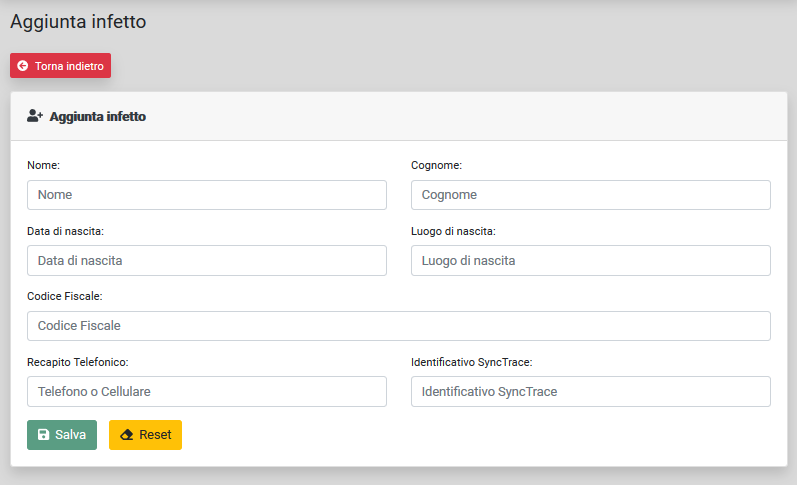
\includegraphics[width=1.0\textwidth]{./immagini/webapp_infected}
\end{figure}
\FloatBarrier

Al momento del salvataggio dei dati presenti nel form, deve essere effettuata una chiamata al metodo \textit{setInfected} dello \textit{smart contract}.
Come mostrato nell'implementazione dello \textit{smart contract}, solo l'\textit{address} dell'admin può chiamare questa funzione. In caso contrario viene lanciata un'eccezione e l'inserimento viene rigettato. Così facendo c'è la certezza che nessuno possa modificare scorrettamente i dati in \textit{blockchain}.\\\\

Per implementare quanto descritto si sfrutta la libreria \textit{web3js}, con i seguenti import:

\begin{lstlisting}
import Web3 from 'web3';
import * as eth from 'ethereumjs-tx';
const Tx = eth.Transaction;
\end{lstlisting}

Le variabili per configurare il contratto e completare correttamente le transazioni in \textit{Ethereum} sono le seguenti:
\begin{lstlisting}
    private web3 = new Web3(new Web3.providers.HttpProvider('https://ropsten.infura.io/v3/YOUR_INFURA_ID'));
    private adminAddress = 'ADMIN_ADDRESS';
    private privKey = environment.BC_PRIVATE_KEY;
    private contractAddress = ''CONTRACT_ADDRESS;
    private abiContract = 'CONTRACT_ABI'
    private myContract = new this.web3.eth.Contract(JSON.parse(this.abiContract), this.contractAddress);
\end{lstlisting}

\textit{web3} è un'istanza utilizzata per fornire un client eseguito tramite il provider Infura.\\
\textit{adminAddress} è l'indirizzo di chi ha effettuato il \textit{deployment}, l'unico con l'autorità per chiamare la funzione \textit{setInfected}.\\
\textit{privKey} rappresenta la chiave privata dell'admin.\\
\textit{contractAddress} è l'indirizzo in cui risiede il contratto nella \textit{blockchain}.\\
\textit{abiContract} è il contratto in formato abi, necessario per creare l'instanza del contratto \textit{myContract}, insieme all'indirizzo del contratto.\\

Per inviare la transazione in \textit{Ethereum} è presente la seguente funzione, che prende in input i dati e effettua la transazione grazie alla funzione di web3js:

\begin{lstlisting}
  sendSigned(txData, cb) {
    const privateKey = Buffer.from(this.privKey, 'hex');
    const transaction = new Tx(txData, {chain: 'ropsten'});
    transaction.sign(privateKey);
    const serializedTx = transaction.serialize().toString('hex');
    this.web3.eth.sendSignedTransaction('0x' + serializedTx, cb);
  }
\end{lstlisting}

Infine, le seguenti righe di codice si occupano di creare i dati della transazione chiamando il metodo \textit{setInfected} per poi inviare la transazione sfruttando la funzione \textit{sendSigned}:
\begin{lstlisting}

  createInfected(infected: Infected) {

    const myData = this.myContract.methods.setInfected( infected.infected_id, true).encodeABI();

    this.web3.eth.getTransactionCount(this.addressFrom).then(txCount => {

      const txData = {
        nonce: this.web3.utils.toHex(txCount),
        gasLimit: this.web3.utils.toHex(GAS_LIMIT),
        gasPrice: this.web3.utils.toHex(GAS_PRICE),
        to: this.contractAddress,
        from: this.adminAddress,
        value: this.web3.utils.toHex(this.web3.utils.toWei('0', 'wei')),
        data: myData
      };

      this.sendSigned(txData, (err, result) => {
        if (err) {
           return console.log('error', err);
        }
        console.log('sent', result);
      });
  }
\end{lstlisting}

Dopo questa serie di operazioni, il codice identificativo della persona inserita tramite interfaccia web, viene segnalato come infetto in \textit{blockchain} e, dall'applicazione mobile, gli utenti che hanno registrato un contatto con l'identificativo segnalato verranno avvertiti di conseguenza.

             % Integrazione con synctrace
% !TEX encoding = UTF-8
% !TEX TS-program = pdflatex
% !TEX root = ../tesi.tex

%**************************************************************
\chapter{Conclusioni}
\label{cap:conclusioni}

%**************************************************************
\section{Raggiungimento degli obiettivi}
Nella sezione \hyperref[sec:obiettivi]{2.4.4} sono stati presentati gli obiettivi proposti dal tutor aziendale a inizio stage.
Di seguito vengono riportate le tabelle degli obiettivi con il loro stato di completamento
\begin{center}
	\begin{longtable}{| c | p{23em} | c | }
		\caption{Tabella degli obiettivi obbligatori}
		\label{tab:obiettivi-obbligatori}\\
		\hline
		\textbf{Obiettivo} & \centering\textbf{Descrizione} & Stato\\
		\endfirsthead
		\hline
		\textbf{Obiettivo} & \centering\textbf{Descrizione} & Stato\\
		\endhead
		\endfoot
		
		\hline
		O01    & Acquisizione competenze sulle tecnologie blockchain, in particolare Ethereum  & Completato\\
		\hline
		O02    & Capacità di progettazione e analisi di smart contract & Completato\\
		\hline
		O03    & Capacità di raggiungere gli obiettivi richiesti in autonomia, seguendo il programma preventivato) & Completato\\
		\hline
		O04    & Portare a termine l'implementazione di almeno l'80\% degli sviluppi previsti & Completato\\
		\hline
	\end{longtable}
\end{center}

\begin{center}
	\begin{longtable}{| c | p{23em} | c |}
		\caption{Tabella degli obiettivi desiderabili}
		\label{tab:obiettivi-desiderabili}\\
		\hline
		\textbf{Obiettivo} & \centering\textbf{Descrizione} & Stato\\
		\endfirsthead
		\hline
		\textbf{Obiettivo} & \centering\textbf{Descrizione} & Stato\\
		\endhead
		\endfoot
		
		\hline
		D01    & Portare a termine il lavoro di studio della portabilità di Ethereum su dispositivi mobili & Completato\\
		\hline
		D02    & Portare a termine l’implementazione completa degli sviluppi previsti & Completato\\
		\hline
	\end{longtable}
\end{center}
	
\begin{center}
	\begin{longtable}{| c | p{23em} | c |}
		\caption{Tabella degli obiettivi facoltativi}
		\label{tab:obiettivi-facoltativi}\\
		\hline
		\textbf{Obiettivo} & \centering\textbf{Descrizione} & Stato\\
		\endfirsthead
		\hline
		\textbf{Obiettivo} & \centering\textbf{Descrizione} & Stato\\
		\endhead
		\endfoot
		
		\hline
		F01    & Completare l'installazione di un peer su un dispositivo mobile Android & Completato\\
		\hline
	\end{longtable}
\end{center}

%**************************************************************
\section{Conoscenze acquisite}
Le conoscenze acquisite durante lo stage sono molteplici, sia a livello teorico che pratico. 
\paragraph{Blockchain}\mbox{}\\
La prima parte del percorso è stata incentrata sullo studio della tecnologia \textit{blockchain}, in tutte le sue sfaccettature. Essendo un campo mai affrontato durante il percorso universitario e non avendo particolari conoscenze pregresse, ho dedicato particolare attenzione allo studio delle \textit{blockchain}, sia per interesse personale, che per comprendere al meglio i concetti generali su cui lo stage era focalizzato. 
\paragraph{Ethereum e Solidity}\mbox{}\\
La fase successiva ha riguardato lo studio della piattaforma \textit{Ethereum} e di tutti gli strumenti utilizzati per lo sviluppo di \textit{smart contract} per la \textit{blockchain}. Grazie allo studio teorico delle \textit{blockchain}, è stato facile comprendere il funzionamento della famosa piattaforma. Il linguaggio di programmazione utilizzato per gli \textit{smart contract} è stato \textit{Solidity}. A prima vista è risultato facile da comprendere, ma padroneggiare fino in fondo la programmazione nel contesto \textit{blockchain} ha richiesto tempo, soprattutto per quanto riguarda l'ottimizzazione del codice.
\paragraph{Utilizzo smart contract in applicazione mobile e web}\mbox{}\\
Dopo aver sviluppato lo \textit{smart contract} per il \textit{contact tracing}, mi è stato richiesto di integrarlo nelle applicazioni SyncTrace. Farlo è stato molto utile e formativo perché non mi sono limitato a sviluppare uno \textit{smart contract}, ma ho anche imparato a sviluppare un'applicazione decentralizzata sfruttando la \textit{blockchain}. Inoltre l'integrazione ha richiesto la collaborazione con il resto del team. 

%**************************************************************
\section{Valutazione personale}
Il bilancio dello stage effettuato presso Sync Lab è senza dubbio positivo. Gli argomenti trattati mi hanno interessato sin dalla scelta del percorso e non hanno deluso le mie aspettative. La \textit{blockchain} è una tecnologia che si sta enormemente sviluppando negli ultimi anni e questa esperienza è stata un'opportunità perfetta per approfondirla. Sono riuscito a comprendere i pregi e i difetti dello sviluppare un'applicazione decentralizzata al giorno d'oggi, quando conviene e quando no, al di là del caso d'uso affrontato nel progetto. Sicuramente è una tecnologia in continua evoluzione e i prossimi anni possono rappresentare una svolta per questo campo. Sarà molto interessante osservare come il passaggio di \textit{Ethereum} al \textit{Proof of Stake} possa aumentare le opportunità e le potenzialità della \textit{blockchain}.\\ 
Valuto positivamente l'esperienza anche per il rapporto con il mondo del lavoro. Lo stage rappresenta un'occasione per affacciarsi al contesto aziendale, completamente diverso da quello universitario. Purtroppo la pandemia ha costretto l'azienda a svolgere la maggior parte delle attività da remoto e questo ha certamente limitato il valore positivo che il tirocinio può portare. Ciononostante, ho apprezzato l'organizzazione aziendale anche in questo periodo, in particolar modo quando è stato possibile svolgere intere giornate lavorative in presenza.
 


             % Conclusioni
\appendix                               

%**************************************************************
% Materiale finale
%**************************************************************
\backmatter
\printglossary[type=main,style=long,nonumberlist]
\input{inizio-fine/bibliografia}
\end{document}
